\documentclass[12pt,a4paper,twoside,openright]{report}


\usepackage[pdfborder={0 0 0}]{hyperref}    % turns references into hyperlinks
\usepackage[margin=25mm]{geometry}  % adjusts page layout
\usepackage{graphicx}  % allows inclusion of PDF, PNG and JPG images
\usepackage{verbatim}
\usepackage{docmute}   % only needed to allow inclusion of proposal.tex
\usepackage{url}
\usepackage[parfill]{parskip}
\usepackage{booktabs}
\usepackage{fixltx2e}
\usepackage{amsmath}
\usepackage{amsthm}
\usepackage{listings}
\usepackage{array}
\usepackage{caption}
\usepackage{subcaption}
\usepackage[justification={centering}]{caption}
\usepackage{float}
\usepackage{framed}
\usepackage{cleveref}
\usepackage{fancyvrb,newverbs,xcolor}
\usepackage{pgfplots}
\usepackage[subpreambles=true]{standalone}	% to include external pgfplots
\usepgfplotslibrary{external}
\usepackage{mathtools}
\usepackage{makecell}
\usepackage{amssymb}
\usepackage{etex}
\reserveinserts{28}


\tikzexternalize% activate externalization!
\pgfplotsset{compat=newest}


\usepackage[UKenglish]{babel}% Recommended
\usepackage[bibstyle=numeric,citestyle=numeric,backend=biber,natbib=true]{biblatex}
\addbibresource{refs.bib}% Syntax for version >= 1.2


\raggedbottom                           % try to avoid widows and orphans
\sloppy
\clubpenalty1000%
\widowpenalty1000%

\renewcommand{\baselinestretch}{1.1}    % adjust line spacing to make
                                        % more readable

\crefname{section}{\S}{\S\S}
\Crefname{section}{\S}{\S\S}
\crefformat{section}{\S#2#1#3}

  
\lstdefinelanguage{Typescript}{
	keywords={break, case, catch, continue, debugger, default, delete, do, else, finally, for, function, if, in, instanceof, new, return, switch, this, throw, try, typeof, var, void, while, with},
	keywordstyle=\color{blue}\bfseries,
	ndkeywords={interface, class, extends, export, void, number, boolean, throw, implements, import, this},
	ndkeywordstyle=\color{orange}\bfseries,
	identifierstyle=\color{black},
	sensitive=false,
	comment=[l]{//},
	morecomment=[s]{/*}{*/},
	commentstyle=\color{purple}\ttfamily,
	stringstyle=\color{red}\ttfamily,
	morestring=[b]',
	morestring=[b]"
}

\lstnewenvironment{typescript}[2][] {
	\lstset{
		language=Typescript,
		backgroundcolor=\color{cverbbg},
		extendedchars=true,
		basicstyle=\footnotesize\ttfamily,
		showstringspaces=false,
		showspaces=false,
		numbers=left,
		numberstyle=\footnotesize,
		numbersep=9pt,
		tabsize=2,
		breaklines=true,
		showtabs=false,
		captionpos=b,
		caption=#1,
		mathescape=true
	}
} {}


\definecolor{cverbbg}{gray}{0.85}
\newenvironment{cverbatim}
 {\SaveVerbatim{cverb}}
 {\endSaveVerbatim
  \flushleft\fboxrule=0pt\fboxsep=.5em
  \colorbox{cverbbg}{\BUseVerbatim{cverb}}%
  \endflushleft
}
\newenvironment{lcverbatim}
 {\SaveVerbatim{cverb}}
 {\endSaveVerbatim
  \flushleft\fboxrule=0pt\fboxsep=.5em
  \colorbox{cverbbg}{%
    \makebox[\dimexpr\linewidth-2\fboxsep][l]{\BUseVerbatim{cverb}}%
  }
  \endflushleft
}
\newcommand{\ctexttt}[1]{\colorbox{cverbbg}{\texttt{#1}}}
\newverbcommand{\cverb}
  {\setbox\verbbox\hbox\bgroup}
  {\egroup\colorbox{cverbbg}{\box\verbbox}}
  
  
  
\newtheorem{lemma}{Lemma}

  
\definecolor{c1}{RGB}{118,42,131}
\definecolor{c2}{RGB}{175,141,195}
\definecolor{c3}{RGB}{231,212,232}
\definecolor{c4}{RGB}{217,240,211}
\definecolor{c5}{RGB}{127,191,123}
\definecolor{c6}{RGB}{27,120,55}
  
  
\begin{document}




%%%%%%%%%%%%%%%%%%%%%%%%%%%%%%%%%%%%%%%%%%%%%%%%%%%%%%%%%%%%%%%%%%%%%%%%
% Title


\rightline{\LARGE \textbf{Joshua Send}}

\vspace*{60mm}
\begin{center}
\Huge
\textbf{Conflict Free Document Editing with Different Technologies} \\[5mm]
Computer Science Tripos -- Part II \\[5mm]
Trinity Hall \\[5mm]
\today  % today's date
\end{center}

%%%%%%%%%%%%%%%%%%%%%%%%%%%%%%%%%%%%%%%%%%%%%%%%%%%%%%%%%%%%%%%%%%%%%%%%%%%%%%
% Proforma, table of contents and list of figures

\pagestyle{plain}

\chapter*{Proforma}

{\large
\begin{tabular}{ll}
Name:               & \bf Joshua Send                       \\
College:            & \bf Trinity Hall                     \\
Project Title:      & \makecell[tl]{\bf Conflict Free Document Editing with \\ \bf Different Technologies}\\
Examination:        & \bf Computer Science Tripos -- Part II, June 2017  \\
Word Count:         & \bf 11825			\\
Project Originator: & Joshua Send                    \\
Supervisor:         & Stephan Kollmann                    \\ 
\end{tabular}
}


\section*{Original Aims of the Project}

To design, test, and analyze a collaborative text editor using convergent replicated data type (CRDT) in comparison to a text editor implemented with operational transformations (OT). The CRDT-based system communicates through a simulated network, while the OT-based system is built around the existing Javascript library ShareJS and utilizes a standard network stack. The relative efficiency of various aspects is compared by running a series of experiments on both systems.


\section*{Work Completed}

The main success criteria listed in the proposal have been fulfilled. The system I built implements a thoroughly tested CRDT for text editing on top of a general network simulation delivering packets across an arbitrarily defined topology. In addition, I completed an optional extension adding undo and redo functionality to my CRDT, which has not been done before. The alternative system built around ShareJS was adapted to run the same experiments as my custom implementation. The results show the strength of my CRDT in highly concurrent and replicated situations, while ShareJS has the advantage in very large text documents.

\section*{Special Difficulties}

None.
 
\newpage
\section*{Declaration}

I, Joshua Send of Trinity Hall, being a candidate for Part II of the Computer
Science Tripos, hereby declare that this dissertation and the work described in it are my own work,
unaided except as may be specified below, and that the dissertation
does not contain material that has already been used to any substantial
extent for a comparable purpose.

\bigskip
\leftline{Signed }

\medskip
\leftline{Date }

\tableofcontents

\listoffigures

\listoftables

\newpage
\section*{Acknowledgements}

I would like to thank the following people for their helpful and enthusiastic contributions to this project:

\begin{itemize}
	\item{\textbf{Stephan Kollmann,} for continual support and guidance throughout the project and for often hinting at ideas I may have missed and thereby letting me explore and develop my own solutions.}
	
	\item{\textbf{Martin Kleppmann,} for his willingness to help with various aspects of the project, and especially providing the starting point for development of the CRDT.}
	
	\item{\textbf{Joseph Gentle,} for providing the initial idea of implementing a P2P distributed text editor. Though the idea changed in terms of technology, the core idea remained.}
	
	\item{\textbf{Proof Readers} of this document including Prof.~Simon Moore, my family and my friends.}
	
\end{itemize}


%%%%%%%%%%%%%%%%%%%%%%%%%%%%%%%%%%%%%%%%%%%%%%%%%%%%%%%%%%%%%%%%%%%%%%%
% now for the chapters

\pagestyle{headings}

\chapter{Introduction}

Real time interaction between users is becoming an increasingly important feature in many applications, from word processing to CAD to social networking. This dissertation examines trade-offs that should be considered when applying the prevailing technologies that enable lock free, distributed modification of data. More specifically, this project implements and analyzes a concurrent text editor based on Convergent Replicated Data Types (also known as Conflict-free Replicated Data Types), CRDT in short, in comparison to an existing editor exploiting Operational Transformations (OT) as its core technology.


\section{Motivation}

Realtime collaborative editing was first demonstrated in the Mother of All Demos by Douglas Engelbart in 1968~\cite{MotherDemo}. From that time, it took several decades for commercial implementations of such editing systems to appear. Early products were released in the 1990s and the 1989 paper by Gibbs and Ellis~\cite{Ellis1989} marked the beginning of extended research into operational transformations (OT). After almost 20 years of research, OT is a relatively developed field and can be found in commonly available products, though many early algorithms have been shown to have flaws~\cite{oster2005proving}. 

The most familiar OT-based product is probably Google Docs\footnote{https://docs.google.com}, which is generally agreed upon to behave in a predictable and well understood way. Importantly, it follows users' expectations for how a concurrent, multi-user document editor should work. This includes lock-free editing, no loss of data, and the guarantee that everyone converges to the same document once modifications have been exchanged. However, the OT algorithms powering distributed text editing are error prone and require high amounts of processing power, as shown in~\cite{dang2016performance}. Conflict-free replicated data types (CRDTs) offer similar features with simpler theoretical foundations and better performance.

Both CRDTs and OT provide eventual consistency: the guarantee that shared data converges to the same state eventually, as in Google Docs. This relates to a cornerstone of distributed systems, the CAP theorem: one cannot guarantee all three of consistency, availability, and partition-tolerance~\cite{Gilbert2005}. However, relaxing the consistency constraint to eventual consistency enables all three~\cite{zeller2014}. Providing eventual consistency is non-trivial and achieved by both OT and CRDTs at different costs, as explored by this dissertation.

%In a distributed system such as a shared text editor, the CAP theorem states one cannot guarantee all three of consistency, availability, and partition-tolerance~\cite{Gilbert2005}.  

%Both OT and CRDTs achieve the key property of eventual consistencyThe data convergence, or consistency, property mentioned above is the hardest to guarantee --- it is easy to create a system where the last writer wins, but data is lost in the process. In a distributed system such as a shared text editor, the CAP theorem states one cannot guarantee all three of consistency, availability, and partition-tolerance~\cite{Gilbert2005}. However, if we forgo strong consistency guarantees and settle for eventual consistency, we are able provide all three~\cite{zeller2014}. As we will see, achieving eventual consistency is non-trivial and achieved by both OT and CRDTs at different costs.



%Data convergence, or consistency, mentioned above is the hardest to guarantee --- it is easy to create a system where the last writer wins, but data is lost in the process. In a distributed system such as a shared text editor, the CAP theorem states one cannot guarantee all three of consistency, availability, and partition-tolerance~\cite{Gilbert2005}. However, if we forgo strong consistency guarantees and settle for eventual consistency, we are able provide all three~\cite{zeller2014}. As we will see, achieving eventual consistency is non-trivial. Both OT and CRDTs provide this key property of eventual data convergence, and are discussed in detail in the preparation section.

%consistency, property above is the hardest to provide -- it is easy to create a system where the last writer wins, but data is lost in the process. In a distributed system such as a shared text editor, the CAP theorem states one cannot guarantee all three of consistency, availability, and partition-tolerance~\cite{Gilbert2005}. However, if we forgo strong consistency guarantees and settle for eventual consistency, we are able provide all three~\cite{zeller2014}. As we will see, achieving eventual consistency is non-trivial. The two prevailing approaches that enable it, operational transformations and commutative replicated data structures, are discussed in detail in the Preparation section.


\section{Overview}
This project aims to examine the compromises made when implementing highly distributed and concurrent document editing with Convergent Replicated Data Types (CRDTs) versus with Operational Transformations (OT). To do this, I have designed experiments which expose statistics about network and processor usage, memory consumption, and scalability. These experiments are run on a system I created based on a specific CRDT, and on a comparative environment built around the open source library ShareJS that implements OT. The system meets the originally proposed goals of implementing a concurrent text editor based on CRDTs which passes various tests for correctness; quantitative analysis is presented in the Evaluation section. 

In contrast to the OT-based library ShareJS, my system, detailed in \cref{sec:crdt}, runs on a peer to peer network architecture instead of a traditional client-server model. The lack of a server reduces the number of stateful parts in the system, at the expense of more complex networking. I managed this complexity by using a simulated peer to peer network, allowing me to control the precise topology, link latencies, and protocol and to explore advantages and disadvantages of using P2P.

In addition to implementing, testing, and analyzing an editor based on a CRDT, as an extension I also upgraded its functionality to include undo and redo capabilities. I developed two approaches using different semantics and consistency models originally. However, one paper I discovered, which develops Logoot-Undo~\cite{weiss2010undo}, takes a very similar approach and is discussed below.

Part of the challenge of this project was to develop the core CRDT and associated algorithms based only on a high level explanation of the desired functionality provided by Martin Kleppmann, based on a paper by Roh~\cite{roh2011replicated} (described in the next chapter). My solution mirrors and incidentally simplifies some of the work done in the paper, and leads to several interesting possibilities for future work (\cref{sec:futurework}). 

%One extension, adding undo functionality to the CRDT, was also completed. I developed two approaches implementing different semantics and consistency models originally. However, one paper I discovered, which develops Logoot-Undo~\cite{weiss2010undo}, takes a very similar approach and is discussed below.

\chapter{Preparation}


\section{Consistency Models}

	\subsection{Definition of ``Conflict Free''}
	
	There appear to be multiple interpretations of ``conflict free''. On one hand, there is the users' intuitive idea that any of their own operations should behave as if they were the only users on the system. For example, inserting a character at index 9 should result in it appearing and staying at index 9. On the other hand, there is the data-centric view of conflict. In this case, operations conflict if they are concurrent and modify the same data. Two users inserting different characters at index 10 concurrently have made conflicting operations. Conflict free then means that no data is lost, and after all users' operations are exchanged the resulting text agrees.
	
	To demonstrate, in the situation above each user expects their text to appear at index 9. If this were carried out, one writer would win in a classic last-writer-wins scenario. However, to satisfy the data-centric definition, data cannot be lost. The solution is to let one user `win' and insert their characters index 9, and offset the other user's characters to appear later. Both operational transformations and CRDTs achieve this merge in fundamentally different ways. This entire process is demonstrated in Figure \ref{fig:reconcile}.
	
	\begin{figure}[htb]
	\centering
	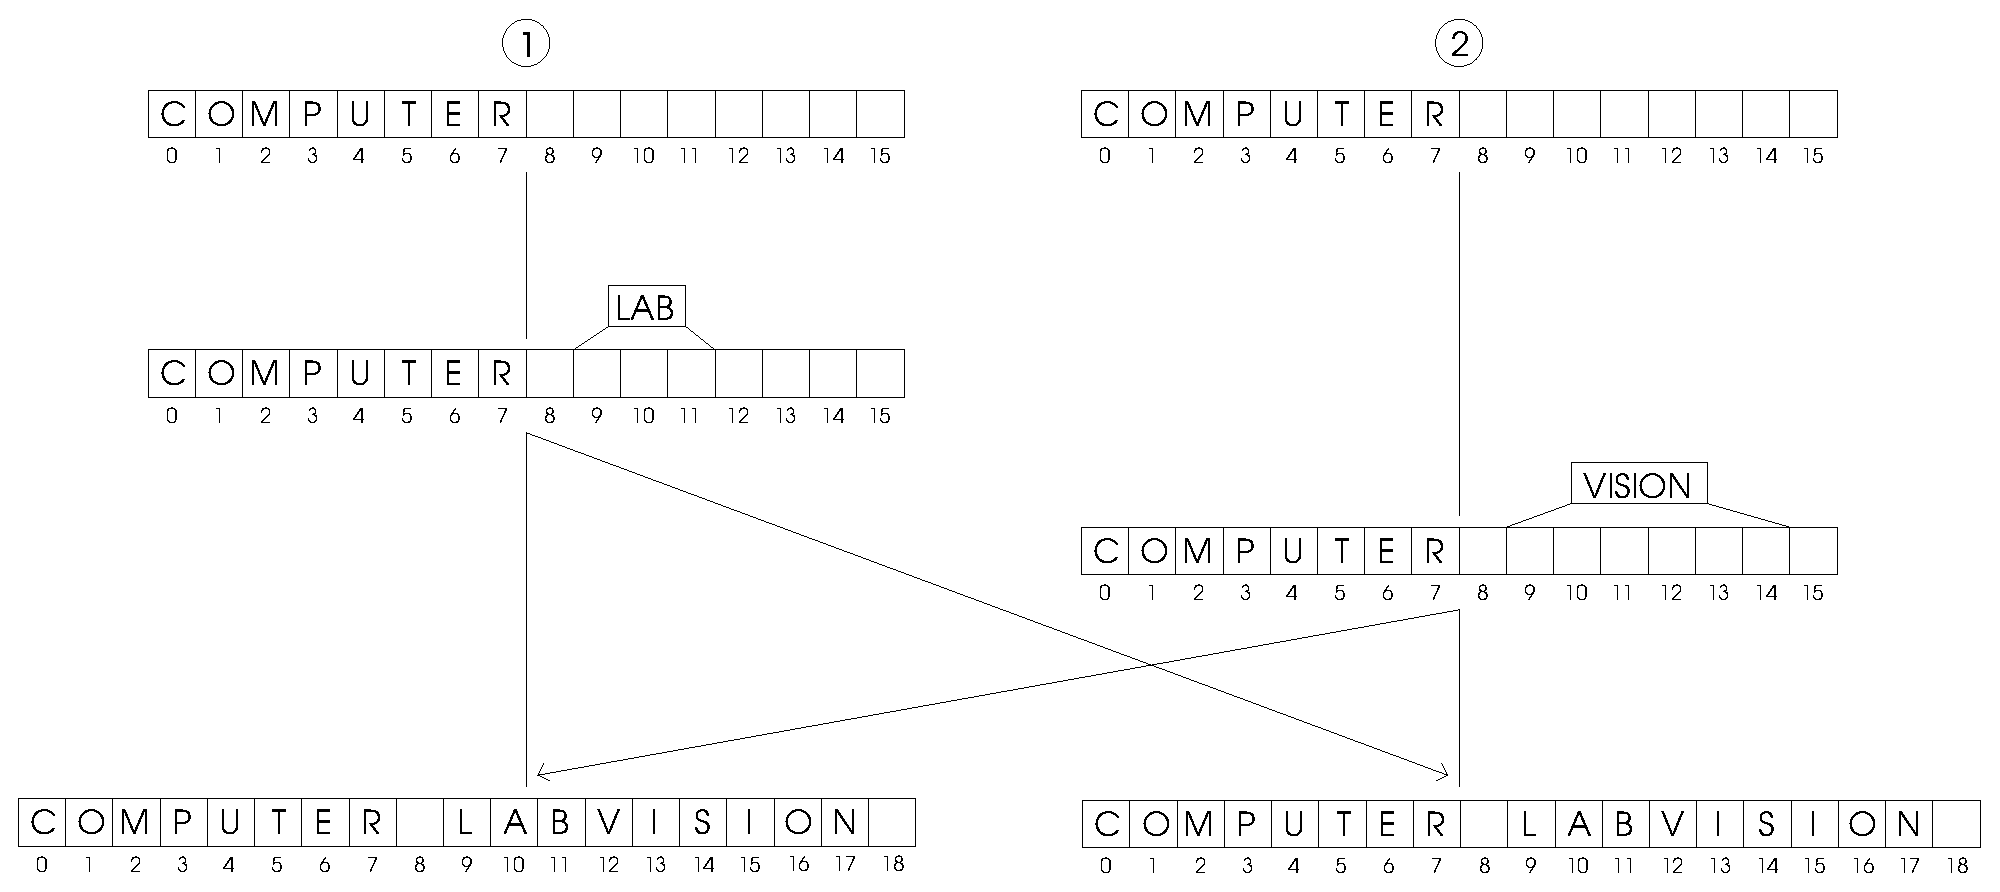
\includegraphics[width=1\linewidth]{figs/reconcile.eps}
	\caption[Achieving Conflict Free Text Editing]{Two clients are initially in a quiescent state i.e. the system has settled with the shared string `computer '. They then concurrently insert different words at the same index. At first each sees only their own edit. Then operations are exchanged and the system reaches quiescence again. Both clients see the string 'computer labvision'. Client 1 thus `won' and kept the original index, while Client 2 had its insertion offset.}
	\label{fig:reconcile}
	\end{figure}
	
	\subsection{CCI Consistency Model} 	\label{sec:cciconsistency}
	The commonly used consistency model for concurrent document editing is the CCI model. The definition here is borrowed from~\cite{weiss2010undo}.
	
	\begin{itemize}
		\item \textbf{Consistency:} All operations ordered by a precedence relation, such as Lamport’s happened-before relation~\cite{lamport1978}, are executed in the same order on every replica.
	
		\item \textbf{Convergence:} The system converges if all replicas are identical when the system is idle.
		
		\item \textbf{Intention Preservation:} The expected effect of an operation should be observed on all replicas. This is commonly accepted to mean:

			\begin{itemize}
				\item \textit{delete}  A deleted line must not appear in the document unless the deletion is undone.
				
				\item \textit{insert}  A line inserted on a peer must appear on every peer and the order relation between the document lines and a newly inserted line must be preserved.
				
				\item  \textit{undo}  Undoing a modification makes the system return to the state it would have reached if this modification was never produced.
				
			\end{itemize}	
		
	\end{itemize}
	
	The given definition of intention preservation is widely used in CRDT development, but may produce some unexpected results as seen when implementing undo functionality in~\cref{sec:cciundo}.
	

\section{Achieving Eventual Consistency}

	\subsection{Operational Transformations}
	
	The easiest way to understand operational transformations is with examples of commonly encountered conflicting operations.
	
	The following figure demonstrates the \textit{concurrent insert at the same index} case, in which two clients at different sites concurrently insert text into the same index in the shared buffer. They key element is the \textit{transform} function which recognizes a local insertion at the same places as the remote one and chooses to offset or not offset it based on client IDs.
	
	\begin{figure}[H]
	\centering
	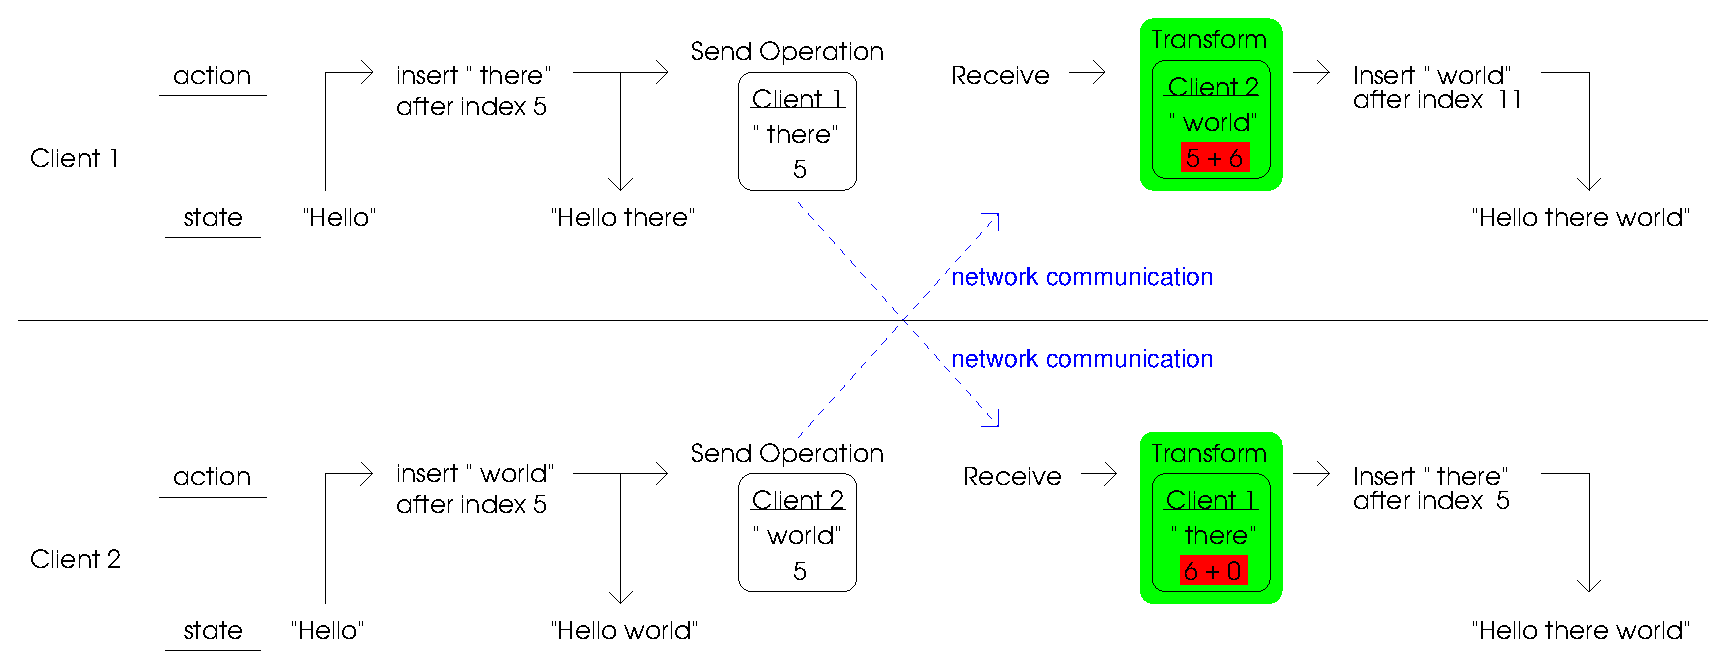
\includegraphics[width=1\linewidth]{figs/ot1.eps}
	\caption[Operational Transformations --- concurrent insertion]{This figure shows how operational transformations might handle concurrent insertion at the same index. Both clients insert different strings after index 5. The operations are exchanged, and the key \textit{transform} function (in green) detects the conflict, and chooses to offset `` world'' on Client 1 by 6 (in red), which is the length of its own previously inserted string `` there''. On Client 2, once the insert `` there'' arrives, the algorithm knows not to offset it (due to some arbitrary ordering such as client ID) and places it at index 5. Thus both clients resolve the string ``Hello there world''}
	\label{fig:ot1}
	\end{figure}
	
	The next figure demonstrates the \textit{concurrent deletion of the same character} case.

	\begin{figure}[H]
	\centering
	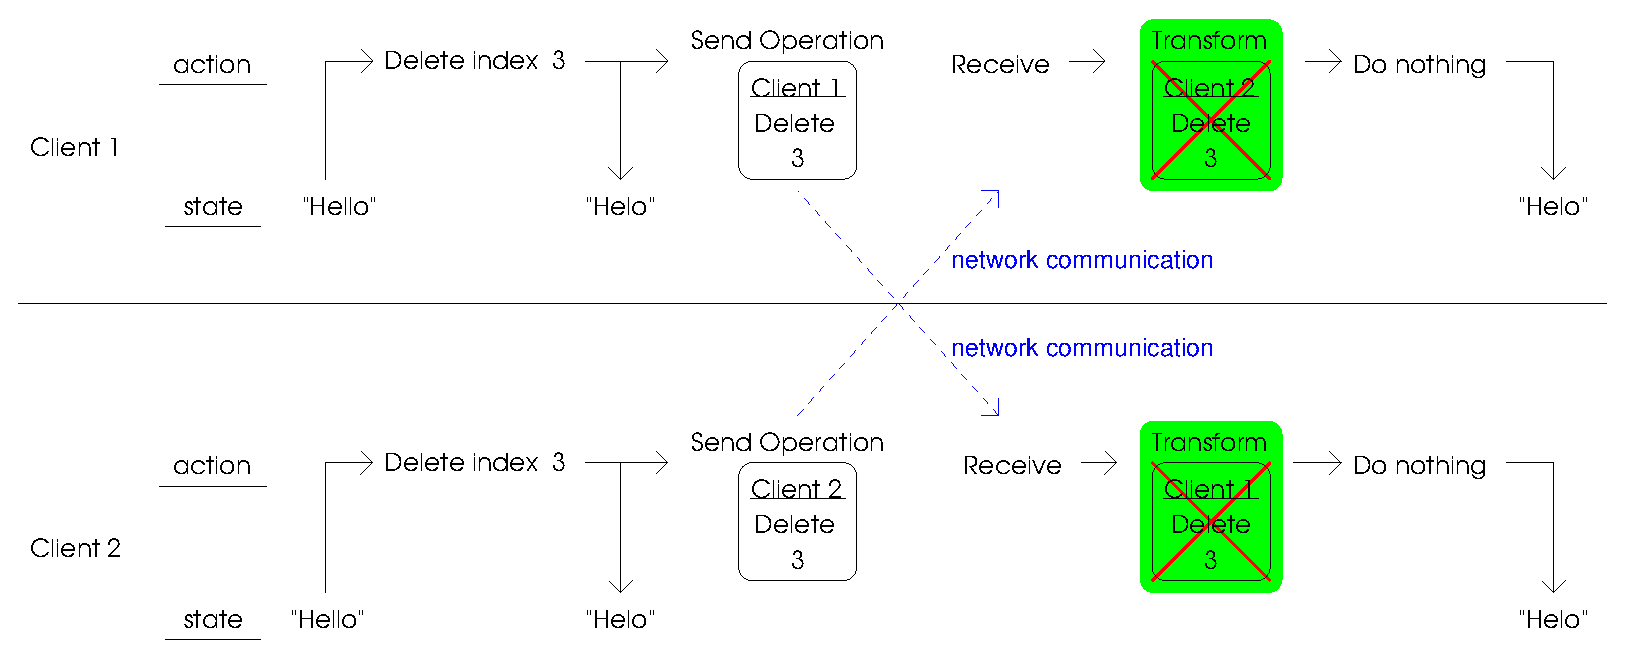
\includegraphics[width=1\linewidth]{figs/ot2.eps}
	\caption[Operational Transformations --- concurrent deletion]{Both clients concurrently delete index 3 of ``Hello'', resulting in ``Helo''. The operations are exchanged. The \textit{transform} function (in green) detects the conflict, and on both clients discards the remote operation. Integrating it would cause modifications the user did not execute (i.e. delete `o' in addition). By discarding the operations, both clients resolve ``Helo'' correctly.}
	\label{fig:ot2}
	\end{figure}
	
	This final figure demonstrates the \textit{concurrent insertion and deletion} case.
	
	\begin{figure}[H]
	\centering
	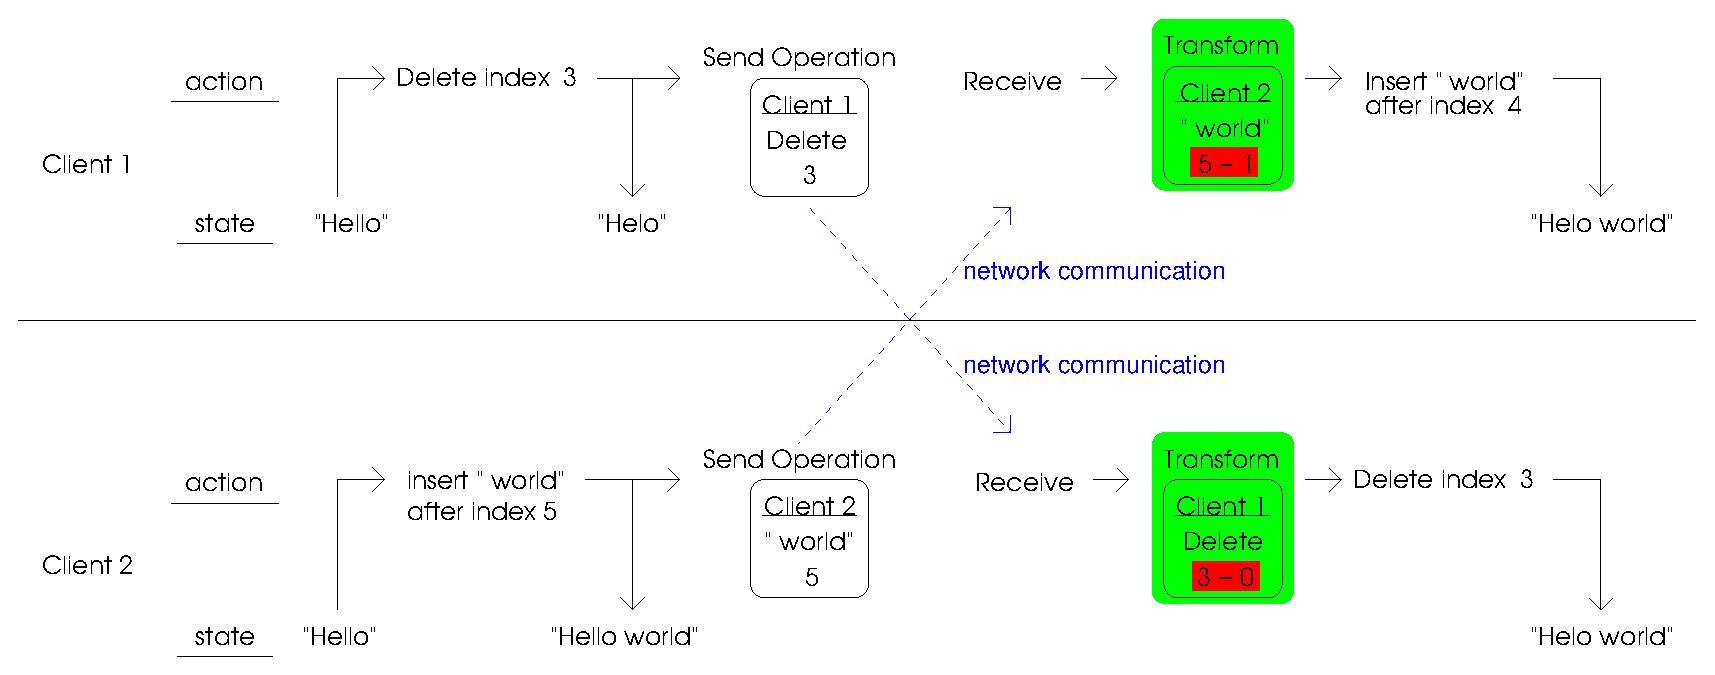
\includegraphics[width=1\linewidth]{figs/ot3.eps}
	\caption[Operational Transformations --- concurrent insertion and deletion]{Client 1 deletes index 3 of the initial string ``Hello'', resulting in ``Helo''. Meanwhile, Client 2 inserts `` world'' after index 5 resulting in ``Hello world''. The operations are exchanged. The \textit{transform} function (in green) detects the conflict, and on Client 1 knows to subtract 1 from the index to insert `` world'' after because a prior character has been deleted concurrently. On Client 2, there is no conflict and the delete can proceed at position 3. Thus both clients resolve ``Helo World'' correctly.}
	\label{fig:ot3}
	\end{figure}

	\subsection{ShareJS} \label{sec:sharejs}
	
	ShareJS~\cite{sharejs} is an open source Javascript library implementing Operational Transformations which can be deployed on web browsers or NodeJS\footnote{\url{https://nodejs.org/en/}} clients. As there are a large variety of algorithms that can enable OT~\cite{kumawat2016}, rather than tracking down the papers ShareJS is based on, much of what is summarized below was deduced by reading its source code. Its core features are shared, versioned documents, an active server which orders and transforms operations, and primary actions \textit{insert} and \textit{delete}.
	
	Each operation applies to a specific document version. The version number is used to detect concurrent changes and transform operations against each other.
	
	An Insert operation for inserting ``Hello World'' at index 100 in document version 1, transmitted as JSON\footnote{JavaScript Object Notation -- a human readable and writable serialization of Javascript objects using maps and lists (\url{http://www.json.org/})}
\begin{lcverbatim}
{v:1, op:[{i:`Hello World', p:100}]}
\end{lcverbatim}

	A deletion of the word ``Hello'' at index 100:
\begin{lcverbatim}
{v:1, op:[{d:`Hello', p:100}]}
\end{lcverbatim}

	Multiple operations may be sent in one packet:
\begin{lcverbatim}
{v:1, op:[{d:`World', p:100}, {i:`Cambridge', p:110}]}
\end{lcverbatim}

\vspace{5mm}

	The library contains both client and a server code. The server provides a serialized order of operations to be applied on each client. The server also transforms concurrent operations against each other, but has the choice of rejecting an operation if the target document version is too old. In order to transform operations against each other, the server must maintain a list of past operations, which is likely to be the primary source of memory consumption. This is confirmed in~\cref{sec:sanitycheck}.
	
	ShareJS clients can only have one packet in flight to the server, which engenders the need for combining multiple operations in a single packet as seen above. This has the implication that as latency increases, the number of packets sent decreases and packet size increases. Clients also must be able to undo operations rejected by the server, as well as transform concurrent, remote operations against local ones. To enable this, clients also buffer past operations. Storing a document of $n$ characters plus a list of at most $m$ operations suggests a space complexity $\Theta (n + m)$.


	\subsection{Convergent Replicated Data Types} \label{sec:crdtoverview}
	
	This section will provide an intuition for CRDTs for text editing in general. The specific CRDT used for this project is mentioned in \cref{sec:rga} and detailed in~\cref{sec:crdt}.

	CRDTs, first formalized in a 2007 paper~\cite{shapiro2007}, trade the complex algorithms used in OT for a more complex data structure. Rather than relying on logic to transform operations against each other, elements are tagged with totally ordered identifiers which allow retrieval of the data in its native form --- for example, a string will be represented as a set of tagged characters and may be read out according to the tag ordering. Figure~\ref{fig:taggedset} is a simple demonstration of how this works. 
	
	\begin{figure}[H]
	\centering
	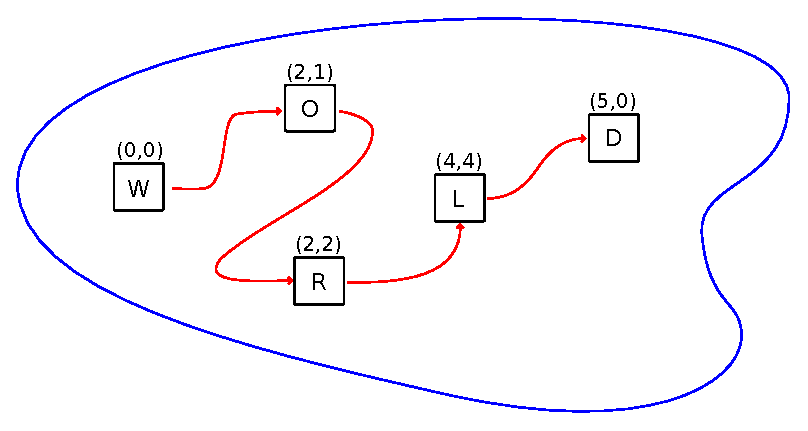
\includegraphics[width=1\linewidth]{figs/tagged_set.eps}
	\caption[Text CRDT as a tagged set]{A generic CRDT containing the word ``World''. The CRDT is a set of nodes tagged with ordered pairs of integers, similar to those used in my CRDT. The ordering is about $<$, first applied to the first element of the pair, then the second. The red arrows trace out the ordering, which presents the word ``World''.}
	\label{fig:taggedset}
	\end{figure}
	
	There are two classes of CRDTs: state- and operation-based. State-based CRDTs disseminate the entire local state to other clients which is then merged into their copies. This requires that the merge operation be commutative, associative, and idempotent~\cite{shapiro2011}. On the other hand, operation-based CRDTs relay modifications to other clients, and require causal delivery between clients, and that concurrent operations commute~\cite{takada2013}. This project uses an operation-based CRDT, so these are the key properties to fulfill.


	\subsection{CRDTs for Text Editing} \label{sec:relatedwork}
		
		I describe a few important CRDTs developed for text editing which demonstrate core ideas used in this project. The RGA CRDT developed by Roh~\cite{roh2011replicated} is discussed only briefly as it mirrors my own implementation and is detailed further in the next chapter.
		
		\subsubsection{RGA}	\label{sec:rga}
		RGA ~\cite{roh2011replicated} stands for replicated growable array. The core ideas developed in the paper are the representation of a character array as a singly-linked list, and the association of each link with a globally unique, totally ordered identifier. The authors use a rather complicated scheme to create these identifiers; the simpler method I develop in \cref{sec:crdt:identifiers} provides the same functionality at lower cost. The paper is quite long and difficult to parse, but ultimately does not offer many practical advances over my independent developments. The authors also make no mention of undo and redo functionality, for which I extend the CRDT in two different ways.
		
		\subsubsection{Treedoc}
		
		Treedoc~\cite{preguica2009} represents a text buffer as a tree structure in which paths from the root are used to encode identifiers and order elements in the set. Nodes in the tree contain at least one character, and the string contained in the buffer is retrieved using infix traversal. Each client can insert a character tagged with a client ID into a local replica of the tree at any time. Two concurrent inserts at the same node are merged as two `mini-nodes' within one tree node. Infix traversal combined with an ordering over the client identifier creates a total order over the characters contained in the tree, including those grouped as mini-nodes. With the total order, all clients can retrieve the same string from their Treedoc replica. Total orders are an important property used to guarantee eventual consistency in text CRDTs. Using unique, ordered client IDs to break ties in concurrent cases is common in CRDT design and indeed used in my own CRDT.
		
		Deletions are handled by marking nodes as removed rather than removing them from the structure, putting Treedoc into the class of \textit{tombstone} CRDTs.
		
		\begin{figure}[htb]
		\centering
		  \begin{tabular}{ >{\centering}m{6cm} >{\centering}m{15mm} >{\centering\arraybackslash}m{6cm} }
		    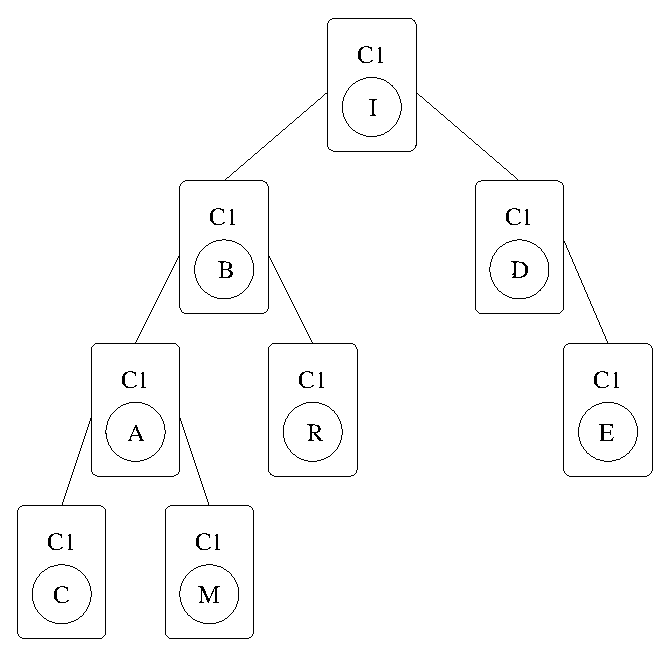
\includegraphics[width=1\linewidth]{figs/treedoc_1.eps}  &
		    $\longrightarrow$  &
		    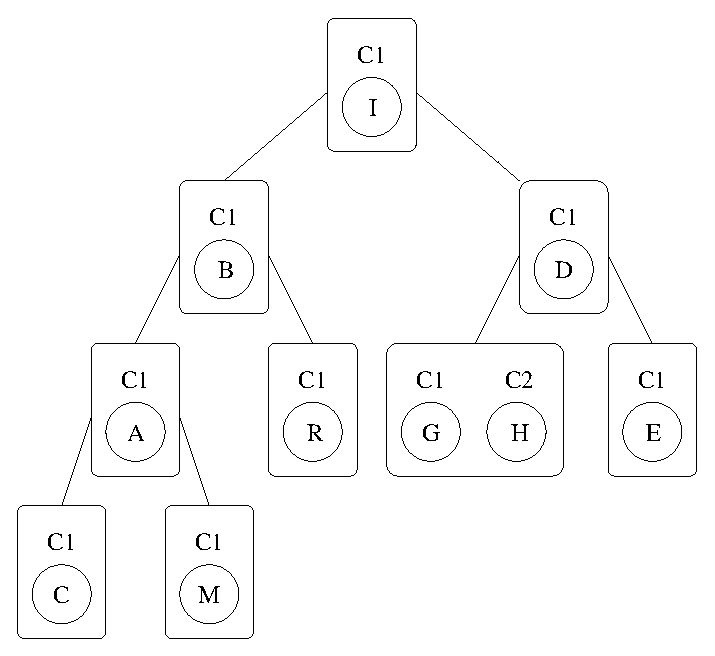
\includegraphics[width=1\linewidth]{figs/treedoc_2.eps}
		  \end{tabular}
		\caption[Concurrent Updates in Treedoc]{Concurrent updates to the same node. In the first state (left), user 1 has written the string `Cambride' into the text buffer. The systems settles and user 2 also sees the string `Cambride'. Both users 1 and 2 realize there is a missing character --- user 1 inserts `g' and user 2 mistakenly inserts `h'. As both create the same node concurrently, they are merged as mini-nodes in the same tree position. Both users now see the string `Cambridghe'.}
		\label{fig:treedoc}
		\end{figure}
		
		\subsubsection{Logoot} \label{sec:logoot}
		
		Logoot~\cite{weiss2008} belongs to the class of text CRDTs that do not require tombstones for deletion. It achieves this by creating totally ordered identifiers without implicit dependencies on other parts of the CRDT (for example, Treedoc nodes depend on the existence of higher nodes in the tree). This means that to delete, any client can simply remove an identifier and the data it tags without adverse effects on the rest of the CRDT.
		
		The process of generating identifiers independently of each other is an expensive process and results in long identifiers. However, the lack of tombstones and improvements made in two further papers~\cite{nedelec2013lseq}~\cite{nedelec2013} provide distinct advantages of prior CRDTs such as Treedoc. Relevant is the idea that identifier generation can be expensive in terms of both space and time: this project uses a simpler identifier scheme.
		
		
		
		\subsubsection{Logoot-Undo} \label{sec:logootundo}
		
		CRDTs generally struggle to provide an undo mechanism since the concept of reversing an update to the data structure breaks causal dependencies. As stated above, Logoot does not embed such dependencies in the CRDT, so implementing an undo and redo as deletion and insertion of a new character and identifier would work. However, this mechanism fails in a concurrent case: two users delete a character concurrently, then undo its insertion independently. The character would appear twice, which is incorrect.
		
		%If it did, the insertion of a character followed by its removal would produce the same result as removal followed by its insertion. In the first case, the character is removed. In the second case, the removal has no effect since the character does not exist yet, so the following insertion takes effect and the character is visible. Thus the order of operations matters; they do not commute.
		
		Logoot Undo~\cite{weiss2010undo} solves this by essentially tagging each character with a $visible$ counter. An undo of an insertion decrements it, while redo increments it. Only if the counter is positive is the character shown. As discussed in~\cref{sec:cciundo}, this leads to some rather unexpected behavior. However, this approach is viable since increments and decrements commute and guarantee eventual convergence. The use of a counter is identical to one undo mechanism I developed independently, though I chose to implement a local undo, only affecting locally generated changes, rather than a global one presented in the paper, which allows any client to undo any other clients' operations.


	
\section{Starting Point}

As stated in the proposal, I had prior experience with ShareJS, which was used as the basis of the comparison system. Additionally, I already had some knowledge of Typescript, my main implementation language. However, almost all other aspects of the project were new to me.

As the project progressed, several courses contributed or reaffirmed ideas I could use. Notably, the Computer Systems Modeling~\cite{compsysmodeling} course had a section on simulation which aligned very well with what I had already implemented at the time. The Part IB course on Concurrent and Distributed Systems~\cite{concdistsystems} provided valuable background towards Lamport and Vector clocks, causality, and total orderings in distributed systems; the IB Computer Networking course~\cite{computernetworking} gave me a solid foundation for planning the network component of my system.


%Lastly, the Mobile and Sensor Systems course\footnote{\url{http://www.cl.cam.ac.uk/teaching/1617/MobSensSys/}} gave me some ideas when seeking alternatives to the flooding implemented in my network simulation.

\section{Requirements Analysis}
To reiterate the success criteria listed in the project proposal, I hoped to

\begin{enumerate}
\item Implement a concurrent, distributed text editor based on CRDTs 
\item Pass correctness tests for this CRDT
\item Obtain and compare quantitative results from ShareJS- and CRDT-based systems
\end{enumerate}

Points one and three have multiple subgoals. For clarity, Table~\ref{table: goals} lists these and their respective importance and difficulty. The completed extension is included as well.

\begin{center}
\begin{table}[H]
\centering
\caption{Project (Sub)goals, priority, and difficulty}
\label{table: goals}
\begin{tabular}{@{}lll@{}}
Goal											 	& Priority & Difficulty \\ \toprule
Implement and unit test core CRDT                	& High     & Medium \\ \midrule
Implement network simulation                     	& High     & High   \\ \midrule
Optimize CRDT Insert                             	& Low      & Low    \\ \midrule
Design experiment format                         	& High     & Low    \\ \midrule
Create comparative ShareJS system					& High     & Medium \\ \midrule
Write log analysis scripts                       	& Medium   & Low    \\ \midrule
Extension: Undo/Redo capability						& Low	   & High 	\\ \bottomrule
\end{tabular}
\end{table}
\end{center}



\section{Software Engineering}

	\subsection{Libraries}
	ShareJS~\cite{sharejs} v0.6.3 (MIT licensed) is the main external resource I required. This package was installed via the NPM\footnote{\url{https://www.npmjs.com/}} package manager. The other external library I used was D3.js\footnote{\url{https://d3js.org/}}, a data visualization tool that helped me build a dynamic network graph for debugging purposes.
	
	\subsection{Languages and Tooling}
	The three main implementation languages, by lines of code, are Typescript\footnote{\url{http://www.typescriptlang.org/}}, Python 2.7\footnote{\url{https://www.python.org/}}, and Coffeescript/Javascript (mainly in ShareJS). I chose Typescript as my primary implementation language because of familiarity, how easily it integrates with web technologies and JSON objects, static typing -- which helps greatly with project scale and early error detection --, and the fact that ShareJS ships as Javascript, which Typescript transpiles to. My development stack included package manager NPM, Typescript, transpiler Babel, and script bundler Webpack; coding was done in Visual Studio Code, an open source IDE developed in parallel with Typescript by Microsoft. How to couple all these tools together correctly is an issue in itself, and setting up a working configuration was one of the most tedious preparation steps.
	
	In order to maximize code reuse and comparability of results both systems must be evaluated on the same platform, a web browser. The most developer friendly choices are Mozilla Firefox\footnote{\url{https://www.mozilla.org/en-US/firefox/new/}} and Google Chrome\footnote{\url{https://www.google.com/chrome/}}, as both come with sophisticated debuggers and script inspection capabilities. I chose Google Chrome as it offers a simple API to obtain heap usage, and its shortcomings in terms of a limited number of active TCP connections are solved with a workaround built into ShareJS.
	
	%\subsection{Tooling}

	
	
	
	%However, both have issues for this project. Firstly, the measuring API for measuring memory consumption in Firefox is complex and badly documented\footnote{\url{https://developer.mozilla.org/en-US/docs/Mozilla/Tech/XPCOM/Reference/Interface/nsIMemoryReporterManager}}. On the other hand, Chrome offers a simple interface to obtain heap usage when certain flags are enabled. Conversely, I discovered Chrome does not allow more than 6 active TCP sessions to a single domain, which I needed to do when running an experiment with more than 6 clients in one browser tab. Firefox has a simple \textit{about:config} setting where this limit can be increased. Luckily, ShareJS contains a built in workaround for the TCP limit most browsers have. Thus with memory measurement support and a solution to the TCP limit, my platform of choice is Google Chrome version 56.
	
	%Before starting this project, I had already been exposed to a specific Typescript development environment and stack. This includes package manager NPM, Typescript, transpiler Babel, and script bundler Webpack, while coding in Visual Studio Code, an open source IDE largely developed alongside Typescript by Microsoft. How to couple all these tools together correctly is an issue in itself, and setting up a working configuration was one of the most tedious preparation steps.
	
	\subsection{Backup Strategy and Development Machine}
	Github\footnote{\url{github.com}} provided the primary backup, with Dropbox also continually backed up to the cloud. To prevent data loss in event of operating system failure, the primary development OS Ubuntu 14.04 LTS x64, backup OS Windows 10, and user data each reside on their own hard drives. The MCS computers were the alternative in case of loss of laptop.
	
	
\section{Early Design Decisions}
%From the outset, I knew I could make simplifications in some aspects of the project, and would likely need to be more flexible and verbose in others. These design decisions were made at various points throughout the development process, though happily most were made early on and required little subsequent change. 

	\subsection{Network Simulation}
	
	I originally chose to implement a network simulation for the CRDT-based system as it allows me to control the topology, link latencies, and protocol and to explore advantages and disadvantages of using peer-to-peer versus a client-server model (especially the role of the degree of connectedness in a P2P network). In addition, I had very little experience with real P2P network and associated routing algorithms and thought it more worthwhile to learn simulation techniques than delve into networking.
	
	However, I also had no experience with simulations, so I simplified wherever possible. My system assumes the network guarantees in-order delivery and is capable of a broadcast to all peers of a node\footnote{True broadcast is not typically found in Internet applications. For instance, IPv6 phases out broadcast functionality and opts for multicast instead~\cite{RFC2460}}. Note that broadcast, or flooding, has severe implications in terms of network efficiency. Without further measures, it sends $\Theta (n^{2})$ packets in a fully connected network, where $n$ is the number of clients. However, though it has downsides, I use broadcast for its simplicity to simulate on given a network topology, and lack of addressing and sophisticated protocols. In~\cref{sec:networkassumptions} I will relax the need for in order delivery using vector clocks.
	
	%While I simplified the routing significantly, I chose to implement support for arbitrary network topologies and latency specification. This enables examining the role of a key property of P2P networks: their connectedness.
	
	%While the broadcast is a useful simplification, the topology of a P2P network affects a system's functionality nearly as strongly. As this project is somewhat a comparison between P2P and client-server architecture, being able to run experiments over different topologies is important. My initial focus was on a fully connected P2P topology to contrast with the client/server star topology. However, forcing the P2P simulation to run on a star itself is perhaps a more direct comparison. With two topologies to test it is already sensible to have a fully general mechanism for specifying a network, so I chose to provide support for arbitrary topologies and latencies on individual links. 
	
	%To aid debugging and visualization [GB?] I also decided to build a dynamic graphical network representation that could be run in tandem with the simulation.

	\subsection{Data Collection and Logging} \label{sec:datacollectiondecisions}
	
	
	Other important design decisions are more general. One is to measure all packet and data structure sizes in terms of number of characters they require when converted into strings using a standard JSON object to string conversion. This allows fair comparisons between my system and ShareJS, and is the most obvious way to measure the size of a JSON object. Alternatives exist which provide more efficient serializations, such as Protocol Buffers~\cite{protobuf}. However, utilizing a more efficient scheme than ShareJS would make for unfair comparisons.
	
	The second decision is to log network packets on the application layer. That is, rather than intercepting and logging packet information at the operating system level, I log payloads of packets from within the applications. This makes comparisons between network traffic more fair, as one system's packets contain no headers, and the other's have TCP/IP overheads.



\chapter{Implementation} \label{sec:implementation}

This chapter describes the implementation of two real-time editing systems, firstly one based on CRDTs, and secondly one based on ShareJS. Following is an overview of the experiment generation and analysis components that are shared by both systems. Lastly the extension that adds Local Undo capability to the CRDT is discussed.


\section{CRDT-based system} \label{sec:crdt}

	\subsection{Overview}
	The high level components that make up my CRDT-based text editor are the user interface, the CRDT, and the network simulation. Each simulated client owns a local replica of the CRDT, an editable text area, and a simplified network stack. The stack disguises from the client the simulated network I created to transmit packets between clients. This approach aims to ease exchanging the simulation for a peer to peer protocol such as WebRTC\footnote{\url{https://webrtc.org}} at a later date. It also allows separate development of the networking subsystem and the CRDT. Such separation of concerns and independence between subsystems are core principles of software engineering that were adhered to throughout the implementation. Figure~\ref{fig:sysarch} shows the architecture of the whole system. 
	
	Upon interaction with a client's text interface, the CRDT is modified and the operations generated are passed via the network to other clients. Upon receipt, the remote clients integrate the changes into their replicas of the CRDT and update the user interface to reflect the new state. The following sections describe the generation and integration of operations.
	
	\begin{figure}[H]
		\centering
		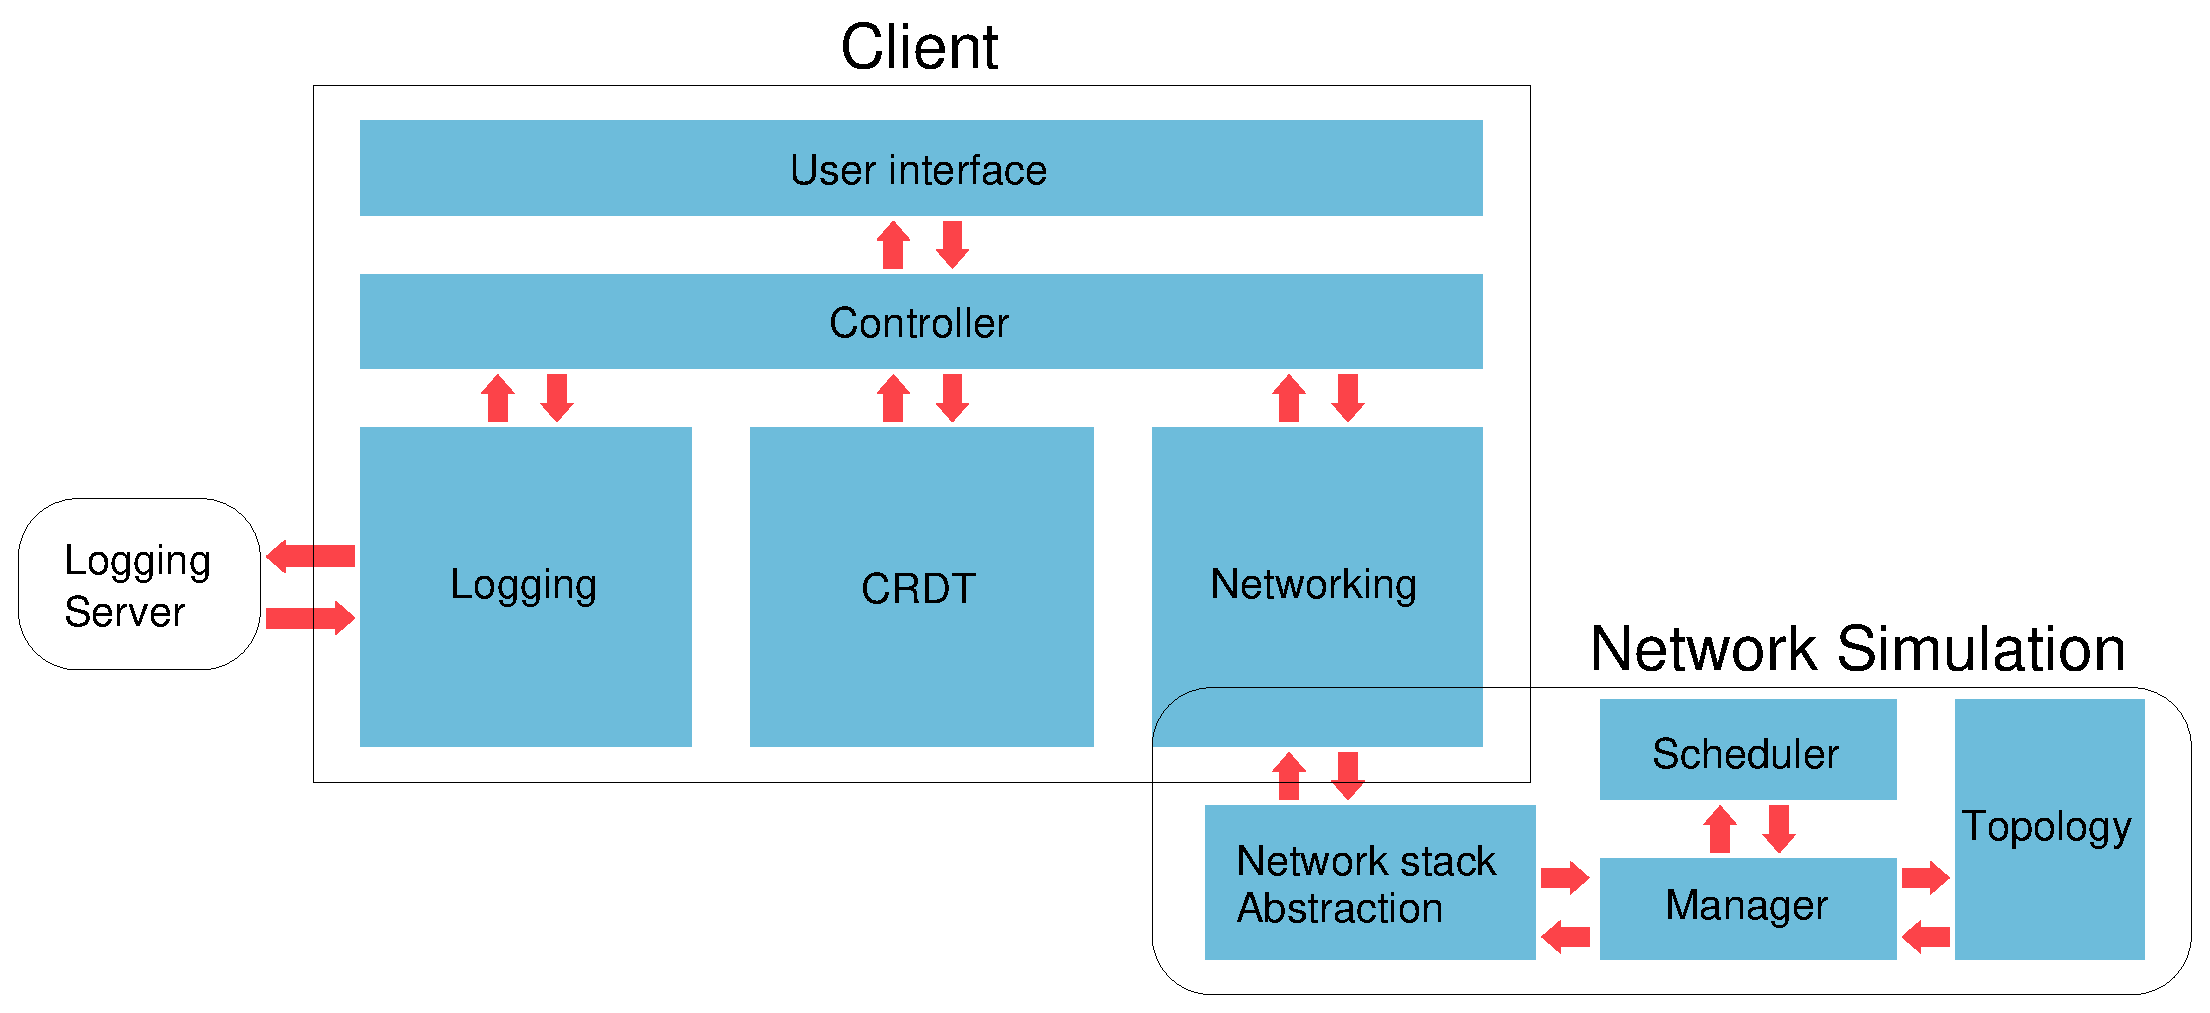
\includegraphics[width=1\linewidth]{figs/sysarch.eps}
		\caption[System Architecture]{An overview of the system architecture implemented for the CRDT-based text editor. Each client has its own UI, controller, CRDT, logger, and networking component. The network module abstracts away the underlying simulation. Many clients can connect to the network abstraction and communicate through it.}
		\label{fig:sysarch}
	\end{figure}
	
	
	\subsection{CRDT}
		To briefly review~\cref{sec:crdtoverview}, a text CRDT can be thought of as a set containing characters tagged with totally ordered identifiers. The document is then extracted in full by ordering the elements according to the total order. 
		
		This subsection goes through the structure and capabilities of the CRDT I utilized, how character identifiers are generated and totally ordered, the operations that are supported in the context of text editing, a brief discussion of tombstones left behind by deletions, and optimizations.
		
		\subsubsection{Structure and Functionality} \label{sec:crdtstructure}
		Previously in~\cref{sec:relatedwork} various CRDTs were mentioned, such as Treedoc which stores characters in the nodes of a tree and retrieves them in infix order. Rather than using a tree to store characters, my approach utilizes a singly-linked list. Each link contains a character $c$, a pointer $n$, and is associated with a unique identifier.
		
		A CRDT needs to implement three core methods in order to support text editing
		\begin{enumerate}
			\item \textbf{Insert:} Add a character at a specific index or location
			\item \textbf{Delete:} Remove or mark as deleted any given character
			\item \textbf{Read:} Retrieve the characters in order and return them as a string
		\end{enumerate} 
		
		
		\begin{figure}[htb]
		\centering
		  \begin{tabular}{ >{\centering}m{6cm} >{\centering}m{15mm} >{\centering\arraybackslash}m{6cm} }
		    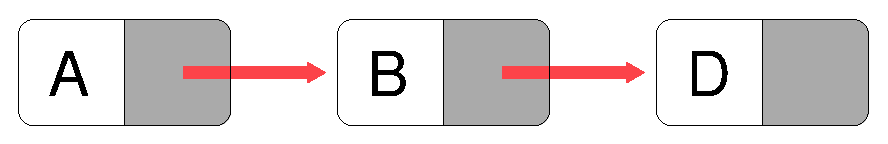
\includegraphics[width=1\linewidth]{figs/linkedlist_0.eps}  &
		    $\longrightarrow$  &
		    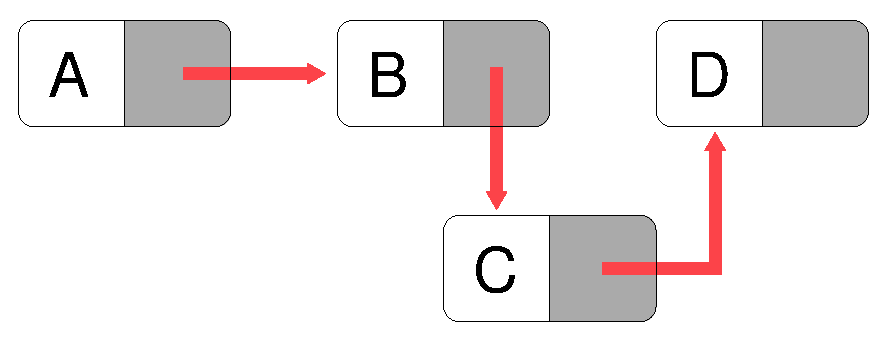
\includegraphics[width=1\linewidth]{figs/linkedlist.eps}
		  \end{tabular}
		\caption[Updating linked lists]{A graphical representation of updating linked lists. Here, a new link containing the character `c' is inserted between `b' and `d' to produce `abcd'.}
		\label{fig:linkedlist}
		\end{figure}
		
		Various data structures were considered when implementing the linked list. The intuitive approach is to implement each link as an instance of a class or structure containing the required identifier, character, and pointer. However, all operations one might want to do on such a linked list are $\Theta (n)$: finding a node to insert after or delete requires scanning some proportion of the list.
		
		A better approach is to implement the linked list within a hash table. Since node identifiers are required to be unique, they can be used as keys in the map and achieve close to constant lookup times and thus fast insert and delete operations. To be more precise, under the assumption of uniform hashing, a hash function is generally $O(m)$ where $m$ is the length of the key. The keys used in my CRDT are of length $\Theta (log(n)+log(r))$ where $n$ is the number of characters in the CRDT and $r$ is the number of replicas in the distributed system. Figure~\ref{fig:hashlist} gives a sample CRDT implemented within a Javascript Object hash map.
		
		
		


%\begin{framed}
%	\begin{lstlisting}
%	{
%	 	"0":	{"n":"7.1","c":""},
%		"1.0":	{"c": " ","n":"2.0"},
%		"2.0":	{"c":"w","n":"3.0"},
%		"3.0":	{"c":"o","n":"4.0"},
%		"4.0":	{"c":"r","n":"5.0"},
%		"5.0":	{"c":"l","n":"6.0"},
%		"6.0":	{"c":"d","n":null},
%		"7.1":	{"c":"H","n":"8.1"},
%		"8.1":	{"c":"e","n":"9.1"},
%		"9.1":	{"c":"l","n":"10.1"},
%		"10.1":	{"c":"l","n":"11.1"},
%		"11.1":	{"c":"o","n":"1.0"}
%	}
%	\end{lstlisting}


	\begin{figure}[H]
		\centering
		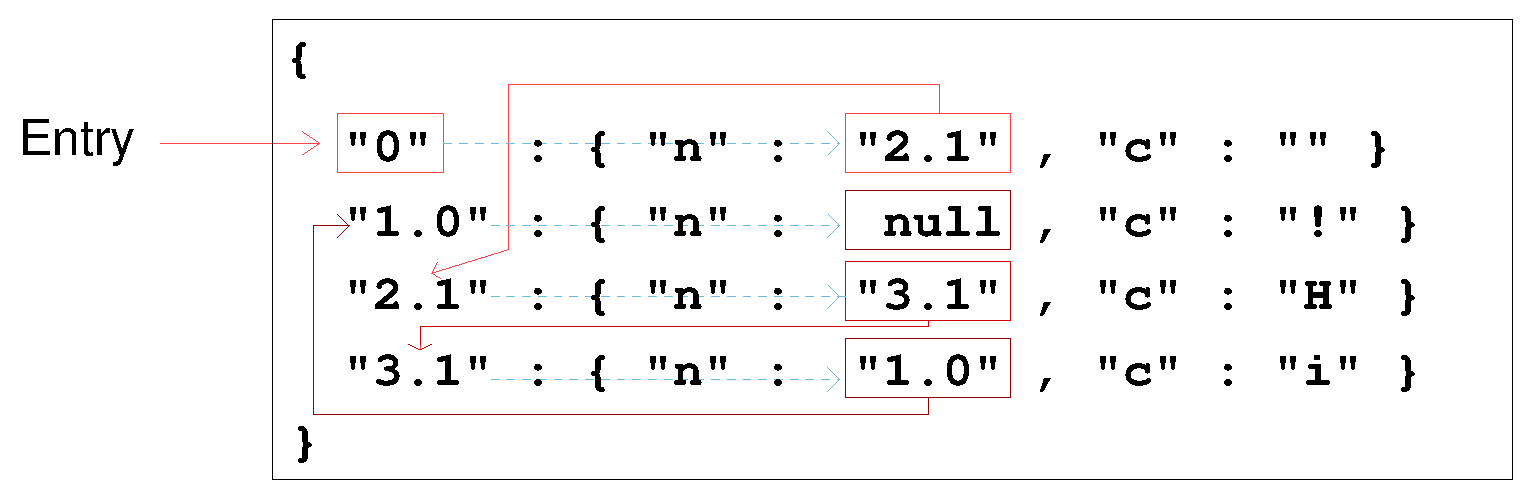
\includegraphics[width=1\linewidth]{figs/json_annotated.eps}
		\caption[Annotated CRDT]{A sample CRDT annotated with arrows. The red arrows denote the links in the linked list. The invariant anchor element tagged `0' is always retrieved first and invisible to the user. The final link, tagged ``1.0'' has no further pointer. Pointers are labeled \texttt{n} in the diagram. The string contained in this instance is ``Hi!''.}
		\label{fig:hashlist}
		\end{figure}
%\ end{framed}
		
		Javascript provides two native objects capable of mapping: Map and standard Javascript Objects. I implemented my CRDT using both structures and eventually settled on native Objects for ease of serialization to JSON and the inconvenience of using Maps: Javascript Maps hash pointers to keys rather than hashing the key contents themselves, making them difficult to work with if pointers are not retained throughout the lifetime of the program.
		
		%Javascript provides two native objects capable of mapping. One is the Map\footnote{\url{https://developer.mozilla.org/en/docs/Web/JavaScript/Reference/Global_Objects/Map}} structure, and another is the standard Javascript Object (referred to as Objects). Both have advantages and disadvantages: Objects only allow strings and numbers to be used as keys, while Maps can use arbitrary entities. On the other hand, Objects serialize very easily to JSON (Javascript Object Notation), while Maps would require their own conversion functions. As we will see in the next section, CRDT keys are pairs of numbers. Thus, the sensible structure would be a Map, as we can map from pairs to values. Unfortunately, Maps natively do not hash the contents of a pair, but only the reference to it. I implemented both Map and Object variants of the CRDT, but was not able to retain original pairs needed for the Map. To solve this issue I serialized the key pair into a string on each lookup and insert which are immutable and thus compared by content rather than pointer. This makes Maps equivalent in functionality to Objects without the JSON serialization. Thus, I eventually settled on CRDTs implemented using Objects as lookup structures.
		
		%For intuitiveness ``linked-list'' will be used instead of ``CRDT'' where helpful.
	
		\subsubsection{Identifiers} 	\label{sec:crdt:identifiers}
				
		Recall that CRDT identifiers are required to be globally unique and totally ordered. My CRDT is advantageous over tree-based CRDTs in that generating identifiers is straightforward. Each client has a unique ID (referred to as \textit{cid}) which forms one part of each identifier. A \textit{cid} can either be randomly generated or provided by the bootstrapping server for the P2P network. In this project, the network simulation provides unique \textit{cid}s.
		
		Define an identifier generated by client $i$ to be a pair $(t_i, cid_i)$ where $t_i$ is a the value of a local counter incremented on every insert. $cid_i$ is the globally unique identifier of $i$. Since each client provides a monotonically increasing $t$ per identifier, and $cid$ is globally unique, every pair generated in the system is guaranteed to be unique.
		
		The counter $t_i$ is maintained as a Lamport clock~\cite{lamport1978}. This means that when receiving an incoming operation with a greater $t_j$ than the local clock, set the value of $t_i$ is set to $t_j$. This guarantees that only concurrent operations can have the same clock value, and is useful when incorporating a remote insert operation into a local CRDT replica.
		
		%This guarantees that any operation that is causally generated after another (defined in more detail later) has a higher clock value, which in turn guarantees that only concurrent operations can have the same clock value. Note that this does not imply that all concurrent operations necessarily have the same clock value. The only meaningful deduction that can be made is that a remote, incoming operation that has a lower $t$ than the local clock, must have been concurrent. This is a key idea utilized when resolving concurrently inserted characters.
		
		I now define a total order $<_{id}$ over the identifiers:
		
		\[(t_1, cid_1) <_{id} (t_2, cid_2) \Leftrightarrow t_1 < t_2 \lor (t_1 = t_2 \land cid_1 < cid_2)\]
		
		
		\subsubsection{Insert Operation}
			Insertion into a text document is one of the two fundamental modifying operations that must be sent to other clients. An insert operation is stored and transmitted as an insert bundle \texttt{B} containing: 
			\begin{itemize}
				\item A unique identifier \texttt{id} for the character
				\item The character \texttt{char}
				\item The unique identifier \texttt{after} of the node after which to insert the character. This corresponds to the position in the linked list at which the character needs to be spliced in.
			\end{itemize}
			
\vspace{3mm}	
\begin{typescript}[Insert Bundle Type Signature][]
interface InsertMessage {
    id: string,
    char: string,
    after: string
}
\end{typescript}
				
				Incorporating an insert bundle \texttt{B} into the CRDT acts according to the following pseudocode.
				
\begin{typescript}[Incorporating Insert Bundle into CRDT][]
 prevNode = map.get(B.after)
 while prevNode.next $>_{id}$ B.id do
   prevNode = map.get(prevNode.next)
 map.add(B.id, Node(B.char, prevNode.next))
 prevNode.next = B.id
\end{typescript}
%				\begin{enumerate}
%					\item Locate in the hash table the node $Prev$ corresponding to the $B.after$ identifier
%					\item While $Prev.next \geq B.id$, do $Prev = get(Prev.next)$. This skips over local concurrently inserted nodes
%					\item Create a new node $Node$, with $Node.char = B.char$ and $Node.next = Prev.next$
%					\item Create a new hash table entry with key $B.id$ and value $Node$ $B.id$
%					\item Rewrite $Prev.next = B.id$ pointer to point to the new $Node$, repairing the linked list
%				\end{enumerate}
				
				This is the standard procedure to insert a new node into a linked list, with the exception of lines 2 and 3. These are the key steps to ensure that all clients converge to the same string, no matter the order the concurrent inserts are incorporated (commutativity property). Figure~\ref{fig:totalorder} demonstrates the effect the \texttt{while} loop: it is enforcing the total ordering defined previously. This ensures all clients incorporate concurrent operations in the same position and hence converge to the same result. The stopping condition ($\not >_{id}$) is enforced by the use of Lamport clocks for identifiers.
				
				
			\begin{figure}[H]
				\centering
				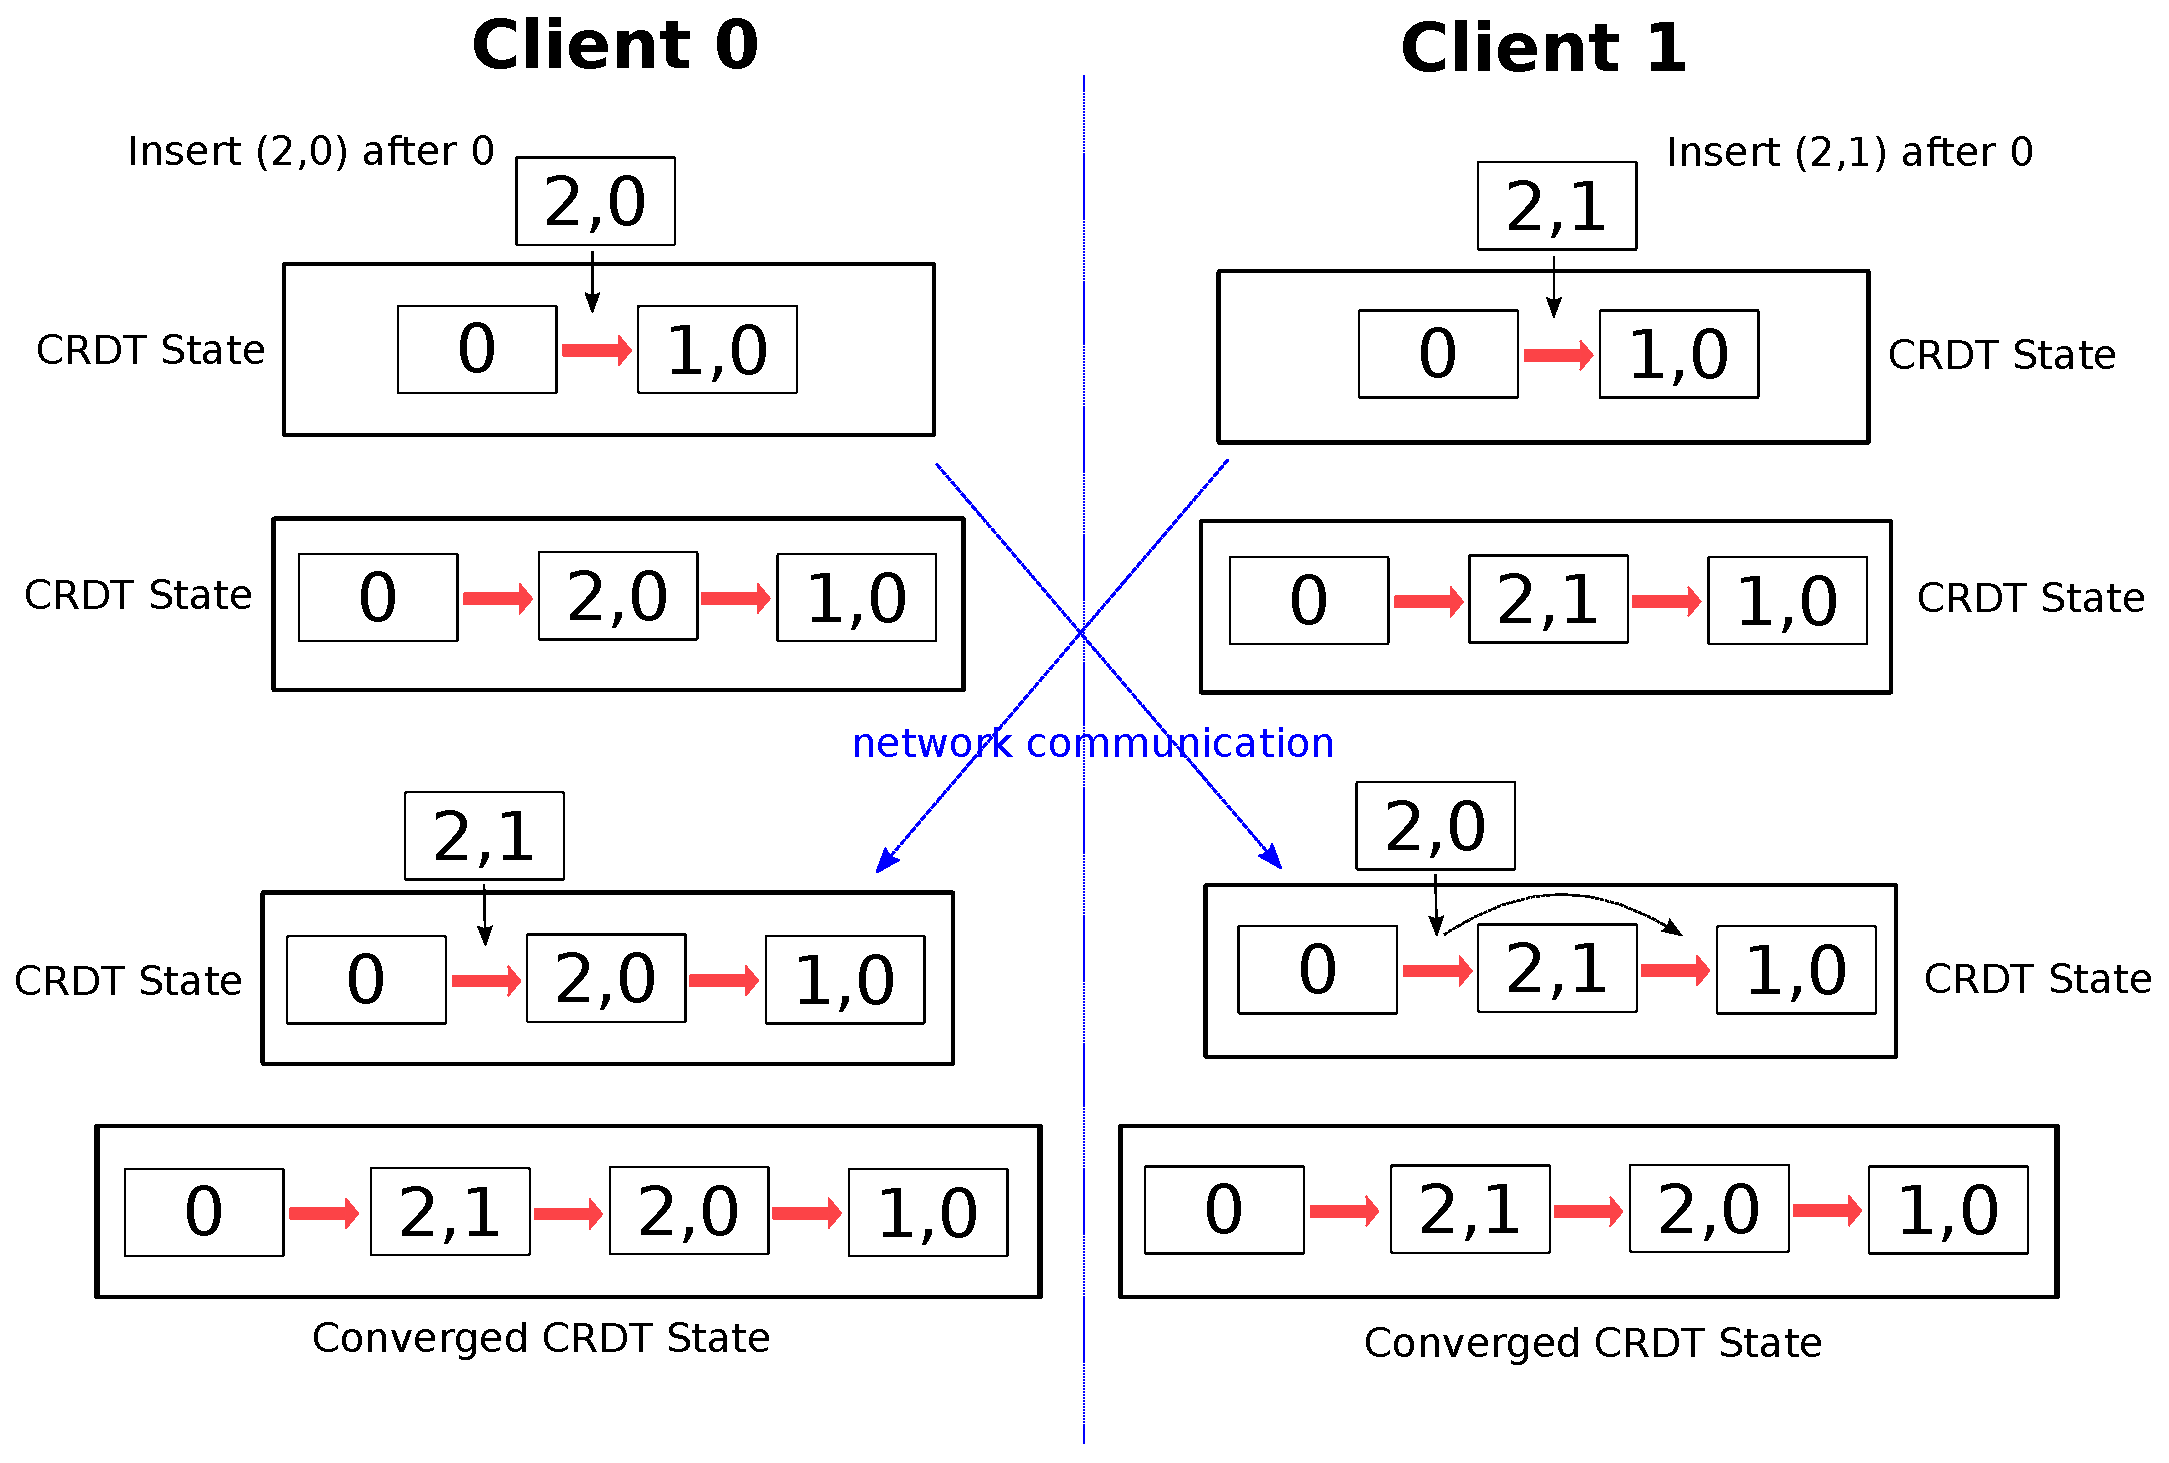
\includegraphics[width=1\linewidth]{figs/totalordering.eps}
				\caption[Convergence using Total Order]{This simplified figure showing only character identifiers demonstrates the use of the total ordering to converge to an identical result on all clients. Two clients concurrently insert after identifier \textit{0}. After exchanging operations, Client 1 inserts the remote \textit{2,0} identifier after its own \textit{2,1} according to the total order defined, while Client 0 inserts \textit{2,1} ahead of its locally generated \textit{2,0}.}
				\label{fig:totalorder}
			\end{figure}
				%To understand the intuition behind why this works, recall the key reason for utilizing a Lamport clock: we can deduce that a remote, incoming identifier \texttt{id$_a$} and some locally generated \texttt{id$_b$}, are concurrent $\iff id_a <_{id} id_b$ . Thus, when incorporating \texttt{id$_a$}, we skip over local, concurrent identifiers until finding one where the condition $<_{id}$ fails and insert there. Reciprocally, once local operations arrive at the sender, the same algorithm will be applied. The arrived operations will have greater identifiers, \texttt{id$_b$}$ >_{id}$ \texttt{id$_a$} (same identifiers of concern as before, just on the other client), and so step 2 will iterate over nothing and insert them before \texttt{id$_a$}. Thus on both clients, \texttt{id$_a$} will be reside after \texttt{id$_b$} in the linked list.
				
			\paragraph{Delete}
				Deleting a character from the text document generates a delete operation, which is transmitted as a bundle \texttt{B} containing
				\begin{itemize}
					\item The target character's identifier to be deleted \texttt{deleteId}
				\end{itemize}
				
\vspace{3mm}
\begin{typescript}[Delete Bundle Type Signature][]
interface DeleteMessage {
    deleteId: string
}
\end{typescript}				
				
				Incorporating a delete bundle into the CRDT is straightforward
				\begin{enumerate}
					\item Locate the node \texttt{N} corresponding to \texttt{B.deleteId}
					\item Set a boolean flag \texttt{N.d} to \texttt{true}
				\end{enumerate}
				
		\subsubsection{Tombstones}
			The delete operation described previously never removes nodes, but leaves them behind as tombstones. Some CRDTs, such as Logoot described in~\cref{sec:logoot}, are structured such that the document is a series of independent nodes, which are arranged solely according to their identifiers. Thus, a node can be fully removed without consequence to other nodes. In my CRDT, each node depends on the prior node in the linked list. Unless we can establish that each client has received and executed a delete operation, we cannot remove a node from the linked list. In general this cannot be assumed as other clients may be executing concurrent edits which depend on that node, are working on a document offline, or on a high latency link.
			
			The process of establishing that each client has received and executed an operation can be achieved using an expensive commitment protocol, which is what is suggested in~\cite{preguica2009}. In effect, the system periodically executes a distributed garbage collection. Removing tombstones may be necessary when the data structure becomes unwieldy, until such a point tombstones are useful in implementing undo functionality for the text editor. This is discussed in section~\cref{sec:undo}. I also discuss an alternative garbage collection scheme in \cref{sec:immundo:cost}.
			
		
		\subsubsection{Optimizations}
			The insert operation produces a bundle which contains exactly one character, one identifier, and the identifier of the node to insert after. The number of operations generated can be cut drastically by allowing an insert bundle to contain a contiguous sequence of characters and a single identifier.
			
			An optimized insert bundle contains
			\begin{itemize}
				\item A unique identifier  $(t, cid)$ for the first character
				\item The character sequence $s$ itself
				\item The node after which to insert the character sequence denoted $(t_{after}, c)$
			\end{itemize}
			
			The receiving CRDT incorporates the bundle by generating a new node for each character $s_i$ with identifier $(t + i, cid)$. The first node is pointed to by $(t_{after}, c)$'s $after$ pointer and each new node points to $(t + (i+1), c)$. The final node has a pointer to the original target of $(t_{after}, c)$. The resulting size of the CRDT is the same as when using multiple unoptimized bundles: this optimization only improves network efficiency.
			
			With the optimization, at best, an entire document could be inserted at once, sending exactly one identifier plus a string of length $n$ in a single packet. A more likely scenario is word-by-word or line-by-line insertion. At worst, we revert to the unoptimized case: $n$ characters and identifiers are sent in $n$ packets. If we assume the network  can send arbitrarily long packets, the application-layer network capacity requirement is $\Theta ((m+log(n)) * n/m)$ = $\Theta (n + nlog(n)/m)$, where $m$ is the average number of characters sent per packet. Written another way this is reduced to between $\Omega (n)$ and $O(nlog(n))$ rather than $\Theta(nlog(n))$. The number of packets sent is reduced to $\Theta(n/m)$, which is desirable since standard protocols such as TCP have high per-packet dissemination overheads.
			
			Another optimization was the renaming of tags and names to be as short as possible (often single characters), shortening the resulting serialized JSON string sent over the network. As discussed before in~\cref{sec:datacollectiondecisions}, alternatives to JSON such as Protocol Buffers would eliminate almost all of these overheads, but this would make comparison with ShareJS less direct.
	
	\subsection{Simulated Network}
	
		This section describes the simulated network I created to deliver operations from one client to another. First, I will detail the initial assumptions I made. This is followed by the abstractions the simulation provides to each client. Next I describe the core difficulty in implementing a simulation: the scheduler. Lastly, I will relax the assumptions made below to more closely mirror real world situations.
		
		Note that the term \textit{simulation} is not exactly correct and \textit{emulation} might be slightly more accurate. However, for simplicity and consistency I will use \textit{simulation}.
		
		\subsubsection{Assumptions} \label{sec:networkassumptions}
		The CRDT I implemented requires that messages be delivered causally~\cite{concdistsystems}. We define the happens-before relation \(a \rightarrow b\) to be true whenever $a$ happens before $b$ on the same process, for example \[\text{Receive Insert ``} Hello \text{''} \rightarrow \text{Insert `` } World \text{'' after ``} Hello \text{''}\]
		We then require that all events ordered by $\rightarrow$ be delivered in a valid ordering according to $\rightarrow$. This is called \textit{Causal Delivery}. $\rightarrow$ is a partial order, since there may be some $A$ and $B$ such that neither $A \rightarrow B$ nor $B \rightarrow A$ holds. Concurrent operations can be delivered in any order since they are guaranteed to commute by the properties of the CRDT.
		
		To justify the causal order delivery requirement, simply take the case of inserting a link into a linked list after a node that does not exist yet: potentially causal operations must be delivered in order. 
		
		\underline{Network Assumptions}. These are guaranteed by the simulation.
		\begin{enumerate}
			\item Unchanging network topology
			\item In-order delivery on any single link in the network
			\item No packets are lost
		\end{enumerate}
		
		Along with this, my implementation of individual clients guarantees:
		\begin{enumerate}
			\item Received packets are forwarded in order, i.e. if $A$ arrives before $B$, then $A$ is forwarded before $B$.
			\item Received packets are flooded to peers before the client generates and broadcasts potentially dependent operations.
		\end{enumerate} 
		
		The simulation and client guarantees provide causal delivery.
		
		\begin{proof}[Proof of Causal Delivery Guarantee]
		
		Assume there is some packet $A$ in the network. A packet $B$ is sent in a causally dependent manner, i.e. $A \rightarrow B$, thus $B$ must be delivered after $A$ on every client in the network. Denote the network node which generated $B$ as $sender_B$.
		
		Proof by induction along any shortest path $p$ from $sender_B$, with induction variable $i$, where $p_i$ is the $i$\textsuperscript{th} hop on $p$ from $sender_B$. The flooding mechanism used in the simulation first delivers packets to every node via the shortest path from a sender as long as the network is static and no packets are lost, which are guaranteed by network assumptions 1 and 3.
		
		Base case, $i = 1$.\\
		As $p_1$ is exactly one hop from $sender_B$, and $sender_B$ must have put the packets onto the link in order by client assumption 2, and packets are delivered in order over any link, $p_1$ must receive the packets in order.
		
		Inductive case, $i = m$.\\
		Assume $p_m$ receives packet $A$, then $B$ i.e. in order. By client assumption 1 (in-order forwarding), and network assumption 2 (in-order delivery on individual links), node $p_{m+1}$ must receive $A$ followed by $B$. Because $p_{m+1}$ also lies on the shortest path, this must be the first delivery to $p_{m+1}$.
		
		This holds over every shortest path through the network, including over all identically long paths to a node. Thus, the network guarantees causally ordered delivery to every node in the network.
		
		
		
%		\begin{proof}[Guarantee of Causal Delivery]
%			Part 1. Assume a single packet $A$ is in the network. In order to generate a second packet $B$ such that $A \rightarrow B$, a client must have received $A$, then sent a packet $B$. This process must send $A$ followed by $B$ to all neighbors by client guarantee 2. Thus causally dependent packets are guaranteed to be sent in order initially.
	%		
%			Part 2. Proof by contradiction.
	%		
%			Assume that at some point in the network, a client receives: $B$ before $A$. Also assume and that $A \rightarrow B$. By Part 1, if $A \rightarrow B$, it must initially have been that $A$ was sent before $B$. This means $B$ overtook $A$ at some point. So, one of the following must have occurred:
	%		
%			The packets were delivered out of order on a single link. This cannot happen by assumption 2 of the network guarantees.
	%		
%			$A$ was lost on a link, $B$ was delivered, and $A$ arrived on a different route. This cannot happen by assumption 3 of the network guarantees.
	%		
%			The topology changed between a client forwarded $A$ and $B$ such that $B$ took a faster route than $A$. This cannot happen by assumption 1 of the network guarantees.
%			
%			A client forwarded $B$ before $A$. This cannot happen by assumption 1 of the client guarantees.
%			
%			All possible ways $B$ could overtake $A$ have been contradicted. Thus, the original assumption must be false. And $B$ can never be received before $A$.
			
			
		 
			
		
			%Proof by contradiction. Assume a client receives some packets $A$ and $B$ and that at some prior point, it must have been the case that $A \rightarrow B$. This implies that somewhere in the network $A$ and $B$ switched order. However, on any individual link, $A$ and $B$ stay in order by network assumption 2 above. At any node, packets cannot switch order either, since the implementation immediately forwards an incoming packet to its neighbors (If a particular client generated $B$, it is put on a link after $A$ by the same condition). Lastly, because the network does not change topology and the protocol is deterministic flooding, packets do not dynamically adjust routes and so any packet that begins in order $A$, then $B$ stays in order $A$, $B$. Thus, in no case can $A$ and $B$ switch order and our assumption must be incorrect. Either $A \rightarrow B$ or it must have been the case that $A \not\rightarrow B$ to begin with. The first case proves our goal and the second is irrelevant.
		\end{proof}
		
		That the network is able to guarantee causal delivery is a strong assumption and cannot be made in reality. I will show in~\cref{sec:causaldelivery} how to relax network assumptions 1 and 2.
		
		%\subsubsection{Abstraction}
		%My network simulation is implemented in two parts: a manager which is shared between all simulated clients, and a Network Interface, of which each client has an instance. The %Network Interface essentially emulates the top of a classic network stack, whereas the manager abstracts away the bottom layers. 

		\subsubsection{Upper Network Abstraction: Network Interface} \label{sec:network:networkinterface}
		My network simulation is implemented in two parts: a manager which is shared between all simulated clients, and a \texttt{Network Interface}, of which each client has an instance. The \texttt{Network Interface}, whose type signature is shown below, essentially replaces the top of a classic network stack, while the manager abstracts aways the bottom layers.
		
\begin{typescript}[NetworkInterface Type Signature][]
interface NetworkInterface {
	isEnabled: () => boolean;
	enable: () => void;
	setClientId: (ClientId) => void;
	setManager: (NetworkManager) => void;
	requestCRDT: (ClientId) => void;
	returnCRDT: (ClientId, MapCRDTStore) => void;
	broadcast: (PreparedPacket) => void;
	receive: (NetworkPacket) => void;
}
\end{typescript}

%		The primary mechanism for disseminating a packet to other clients is via the \lstinline|NetworkInterface.broadcast| method, which in turn calls the \lstinline|broadcast| method of the \lstinline|NetworkManager|. It accepts a \lstinline|PreparedPacket| which is an object that contains a bundle (such as \lstinline|InsertMessage| or \lstinline|DeleteMessage| from section [section ref]) and a tag which the receiver uses to disambiguate the type of the incoming packet. This is required since packets are serialized to strings when sent over the network and all type information is lost in the process.
		The primary packet dissemination method is via the \texttt{NetworkInterface.broadcast} method. It broadcasts a \texttt{PreparedPacket}, which contains a bundle and a tag to disambiguate the type of bundle, as type information is lost during serialization over the network.

\begin{typescript}	[][]
interface PreparedPacket {
	type: "i" | "d" | "reqCRDT" | "retCRDT",    // insert or delete message, or request/return CRDT
	bundle: CRDTTypes.InsertMessage | CRDTTypes.DeleteMessage | RequestCRDTMessage | ReturnCRDTMessage;
}
\end{typescript}
		
		As expected, the bundles are either insert or delete operations. Two other types of bundles that can be sent are\texttt{RequestCRDTMessage} and \texttt{ReturnCRDTMessage}, special messages which clients use when joining the network.
		

		
		\subsubsection{Lower Network Abstraction: Network Manager}
		The lower layers of the network stack are provided by the \texttt{Network Manager}. It has two key methods: \texttt{NetworkManager.transmit(sender, packet)} and \texttt{NetworkManager.unicast(from, to, packet)}. The simulation is given a predefined topology, which contains connectivity and latency information. Thus, when a client's \texttt{NetworkInterface} calls \texttt{NetworkManager.broadcast}, the manager knows which clients are neighbors and corresponding link latencies, and can schedule a delivery event for each. The \texttt{NetworkManager.unicast} is used for point to point, single hop communication when joining the network and requesting or returning copies of CRDTs. This module does the work of the network and data layers of traditional network stacks and abstracts away how packets travel between neighboring clients.
		
		\subsubsection{Joining the Network} \label{sec:networkjoin}
		To make the system more flexible, I added the capability to join the P2P network during simulation. Only the first client gets to create a new CRDT; joining clients request a copy of the CRDT via \texttt{NetworkInterface.RequestCRDTMessage} (see~\cref{sec:network:networkinterface}).
		
		An alternative method to requesting an up-to-date CRDT is to begin with an empty CRDT and replay all subsequent operations on it. This would however be significantly less efficient as it requires all remote clients to store all of their previous operations forever, and joining clients would each have to reintegrate all operations. On the other hand, doing a partial state replay would be simpler: transmit only the missing operations. This is not easily done in my implementation. If a client has an out of date CRDT, it must request an entire new copy via \texttt{NetworkInterface.RequestCRDTMessage}.
		
		At this point it is important to acknowledge that introducing dynamic network joining violates one of the guarantees of~\cref{sec:networkassumptions}. Namely, incorporating new clients over time changes the network topology and thus the guarantee of causal delivery no longer holds. The introduction of vector clocks (in \cref{sec:causaldelivery}) will restore this guarantee.
		
		\subsubsection{Causal Delivery} \label{sec:causaldelivery}
		Until this point, the network has guaranteed causal delivery of packets based on strong assumptions and knowledge of the system implementation. These can be relaxed to allow out of order delivery and dynamic network topologies. This can be done using vector clocks~\cite{fidge1987}.
		
		I introduce an additional network layer, as depicted in Figure \ref{fig:causal}. I make a distinction between receiving and delivering a message. Receiving is the arrival of a message at a client, whereas delivery passes the message up the network stack. Causal delivery guarantees that messages are delivered such that $A \rightarrow B \Rightarrow\ deliver(A)$, $deliver(B)$.
		

	\begin{figure}[H]
	\centering
	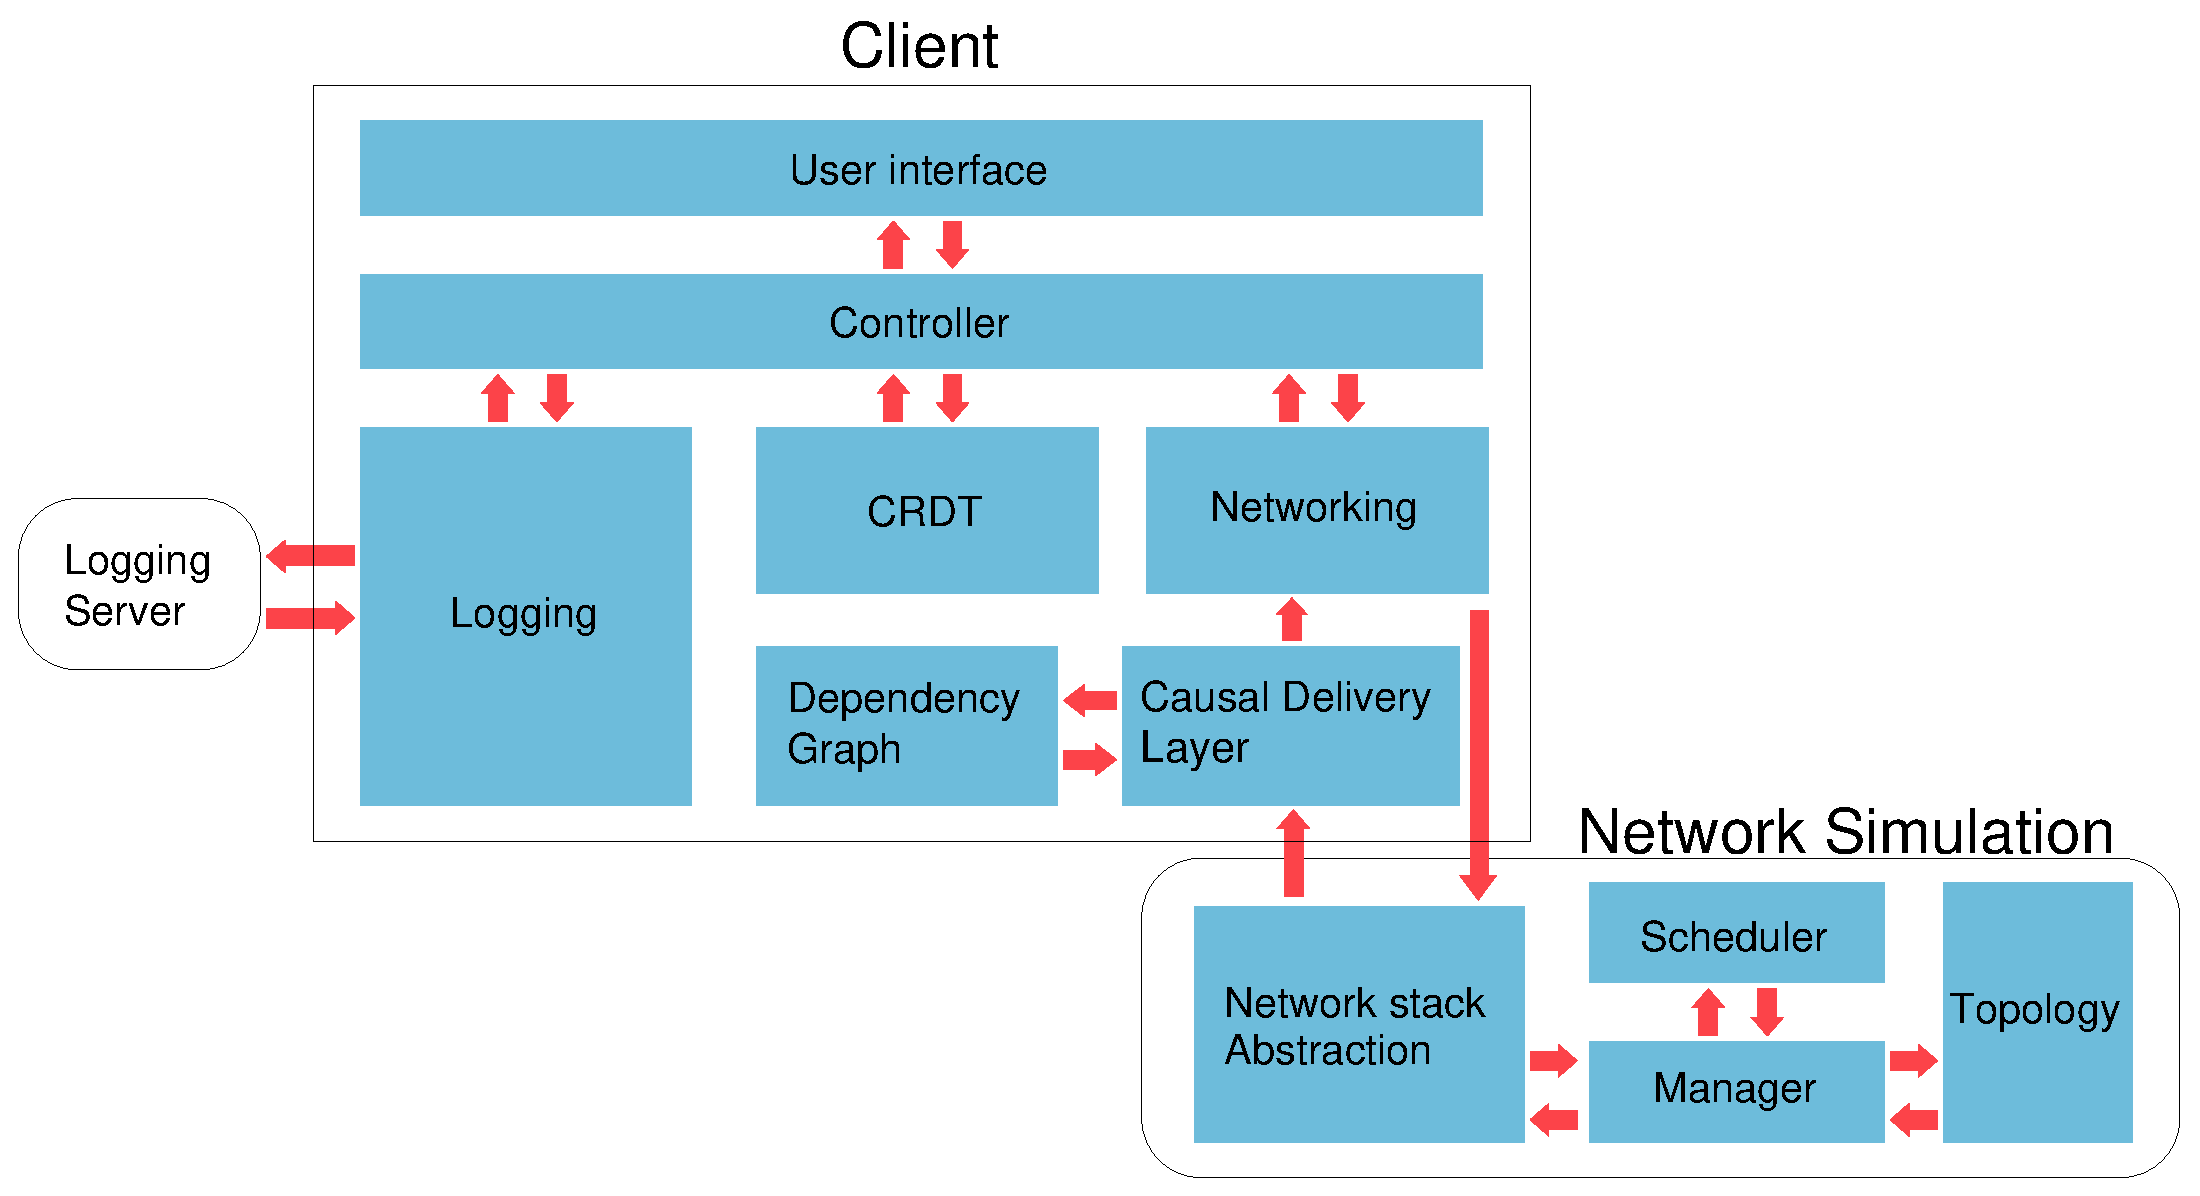
\includegraphics[width=1\linewidth]{figs/causal_arch_2.eps}
	\caption[Ensuring Causal Delivery]{The updated architecture depicting the additional network layer ensuring causal delivery.}
	\label{fig:causal}
	\end{figure}

	
		\paragraph{Modified Vector Clocks} \label{sec:modifiedvectors}
		A traditional vector clock is outlined is Appendix \ref{appendix:vectorclocks}. In this system, the causal delivery layer must delay messages that arrive before all of their causal dependencies are delivered, which requires calculating exactly which messages are missing. To this end, I modified the vector merge rule (number 4 from the appendix) to only increment the local clock whenever a message is generated locally. This way, each value in a vector represents exactly how many messages are known to have been sent by the corresponding client. The full modified rules are listed~\cref{appendix:modifiedvector}.
		
		We can now determine concurrent, causally dependent and causally prior messages by comparing vectors. We define the latter two about $<_v$.
				
		Two vectors $v_1$ and $v_2$ occurred concurrently iff \[\exists c,c' \in v_1,\ v_2.\ v_1.c > v_2.c\ \land\ v_1.c' > v_2.c'\]
		
		Given vectors $v_1$ and $v_2$ with components $v.c$, define \[v_1\ <_v\ v_2 \iff\ \forall c \in v_2, v_2.\ v_1.c \leq v_2.c\ \land\ \exists c' \in v_1, v_2.\ v_1.c' < v_2.c'\]
		We say $v_2$ is \textit{causally dependent} on $v_1$ and $v_1$ is \textit{causally prior} to $v_2$.
		
		If a client receives a vector $v$ that is concurrent with the client's current vector $s$, the causal network layer immediately delivers the message to the client. If $v <_v s$, i.e. is causally prior, then the message has been seen before and can be discarded. If $s <_v v$, i.e. is causally dependent and not seen before, a delta can be computed by taking the element-wise difference between $v$ and $s$, treating missing elements as $0$. This represents the number of messages missing from each client. 
		
		Calculating missing messages is useful in delivering buffered messages. The na\"ive approach is to scan the entire buffer on every packet delivered up the stack, which can result in a cascade of deliveries at quadratic cost. The delta enables building a dependency graph and only checking neighbors of delivered packets for further deliveries.
		
 %		\ref{fig:efficient}.
 %		\begin{figure}[htb]
 %		\centering
 %		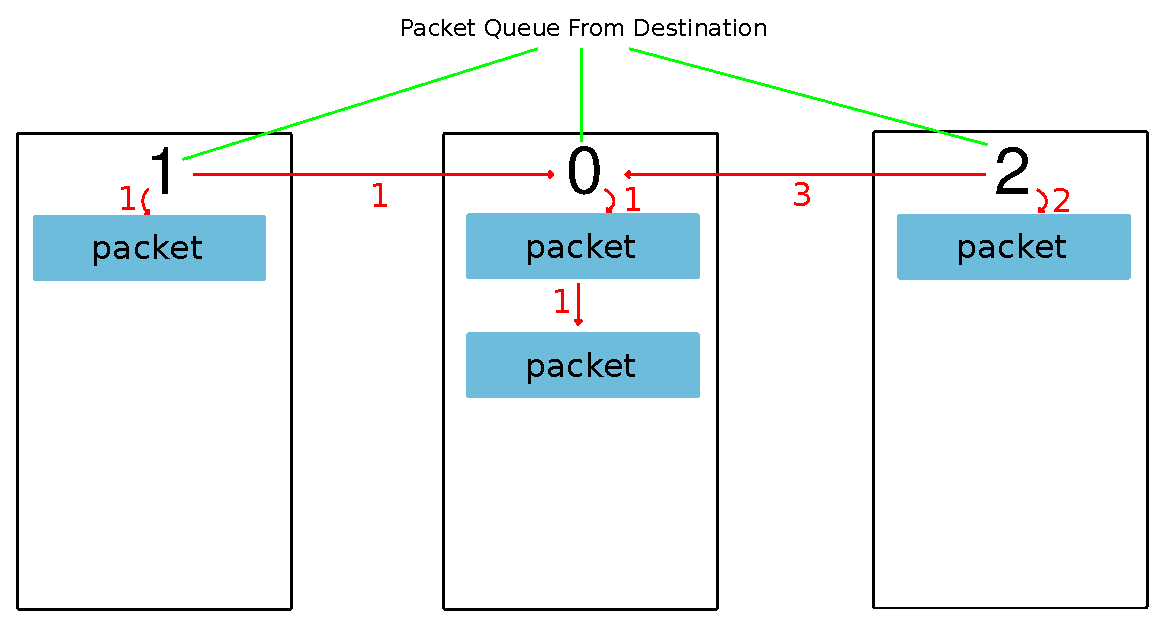
\includegraphics[width=1\linewidth]{figs/efficient_message_buffer.eps}
 %		\caption[Dependency Graph in Message Buffer]{A representation of the graph structure used to efficiently deliver packets. When a new packet arrives from some destination D, all outgoing links from D are decremented. The target of each link checks the head of its queue for potential delivery. The efficiency gain relies on the fact that messages from the same client must be delivered sequentially.}
 %		\label{fig:efficient}
 %		\end{figure}
		
	
	
	\subsection{Simulation}
		A large part of the infrastructure underlying the CRDT is the simulation driving the network and executing preprogrammed events. The core of this is the simulation scheduler which I focus on below. Other components are interfaces to the experimental setup and networking modules.
		
		
		\subsubsection{Scheduler}
	
		A simulation scheduler is responsible for mutating system state based on events to be executed at specific times. To schedule an event, an object needs to call the \texttt{Scheduler.addEvent} method, listed below.
\begin{typescript}[The Scheduler.addEvent method][]
public addEvent(time: number, clock: number, action: any) {
 let heapElem: DualKeyHeapElement = {
     pKey: time,
     sKey: clock,
     payload: action
 };
 this.heap.insert(heapElem);
}
\end{typescript}

		%My scheduler is somewhat more sophisticated than might be expected in that it takes two keys for scheduling: a primary key $pKey$, and a secondary key $sKey$. The need for this arose when submitting multiple packets from a single client at the same time - the original underlying data structure, a heap with a single key, makes no first-in first-out assurances. Thus, packets on a link could arrive out of order, which violated one of the guarantees the network has to provide [reference needed]. To fix this, my scheduler breaks ties using $sKey$, which is a monotonically increasing counter provided by the caller.
		The scheduler uses an underlying heap to manage events, which makes no first-in first-out guarantees. As it is possible for a client to submit multiple packets onto a single link at the same logical time, and~\cref{sec:networkassumptions} requires in-order delivery on any link, my heap uses a secondary key $sKey$ to order delivery.
		
		The key property of a correct scheduler, as noted in the Part II Computer Systems Modeling~\cite[slide 120]{compsysmodeling} course, is that the next executed event be the one with the least remaining time. Using a heap, we get $\Theta (log(n))$ time per element retrieved. Executing an event may generate more events which are added back into the heap.
		%When the simulation is running, the scheduler removes the top event $E$ off the heap, decreases all remaining events' primary keys by $E.pKey$, and executes $E.payload$. This may in turn generate more events which are added back into the heap.
		
		The scheduler is seeded with events defined in an experimental setup, see~\cref{sec:experimentcreation}.
		%Because the simulation needs to be seeded with events and simulated action in order to do anything useful, before letting the execution begin, the scheduler is also used to add a set of mock insert and delete events, which together constitute an experiment. This is discussed in more detail in [section ref]. Once running, its primary use is delivering packets.
		
		\subsubsection{Representation of Time} \label{sec:rtscheduler}
		The concept of time in a simulation is generally taken to be ``logical time''. The system begins at $t = 0$, and each subsequent event moves the $t$ variable forward. This works perfectly well for the network simulation, since the latency on any individual network link is well defined and deterministic.
		
		The alternative `time' that can be used is `wall-clock' time. The amount of time until some next event is given in milliseconds to wait, rather than a logical delta which is skipped over. Using this concept of time in a simulation introduces extra complexity, primarily stemming from inaccuracy in timers provided by the host platform. Indeed, it is likely that some events would have very small deltas, for which starting and stopping a timer would be nearly impossible. 
		%To handle this difficulty, the scheduler runs, in order, all ready events whenever it wakes up rather than just one at a time.
		
		In this project, I implemented both an event-driven scheduler and a timer-driven scheduler. The timer-driven version is useful for debugging and watching the simulation unfold in real time, whereas the event-driven version runs as fast as the hardware permits. However, I found that I could, to an extent, emulate the timer-driven scheduler using the event-driven scheduler by adding a sleep proportional to the $\Delta t$ until the next event. As the event-driven version is more flexible, and simpler -- the driver is a simple while loop, rather than recursively set timers with callbacks -- I decided to use it when executing experiments on the CRDT-based system.
		
		The timer-driven scheduler is still useful in the comparative system (\cref{sec:comparative}), as packet deliveries are nondeterministic.
			
			
\section{ShareJS Comparative Environment} \label{sec:comparative}

	The main difficulty when building the ShareJS-based comparative system was adapting it to allow executing the corresponding experiments to the ones executed in the CRDT-based system. This meant incorporating the real-time scheduler discussed in~\cref{sec:rtscheduler}, and inserting log statements to record data to the logging server.
	
	\subsection{Scheduling}
	An experiment consists, at the most basic level, of a set of simulated events that each client performs at specified times. ShareJS requires that sockets be used to transmit operations between clients, even if they are all on the same machine, which introduces nondeterminism and necessitates using the real time scheduler rather than the logical time one. The scheduler is seeded according to an experimental setup, inserting and deleting characters via hooks available in ShareJS.
	
	The scheduler, logging module, and various helper functions were reused exactly as in the prior system. Their use led to a Typescript/Javascript combined system, but since Typescript is fully compatible with Javascript no major difficulties were encountered, except the lack of type annotations in ShareJS.
	
	\subsection{Logging}
	Enabling data logging primarily consists of inserting log lines at critical points that reveal interesting information about the system. The most important of these are the receiving or sending of any packets from a client or the server, and total memory consumption of the clients before and after the experiment. This was done by reading the ShareJS source code and inserting references to a global logging module at the appropriate points. The server was also modified to log relevant information.
	
\section{Experiment Creation and Use} \label{sec:experimentcreation}

	This section deals with the creation and analysis of the experiments. First I outline the overall system work flow. Then, I discuss the design of an individual experiment. Lastly, I briefly examine the decision to log experiments to text files, then separately parse and analyze these files to collect data.

	\subsection{Work Flow}
	On the whole, this project operates as in Figure~\ref{fig:workflow}. 
	
	\begin{figure}[htb]
	\centering
	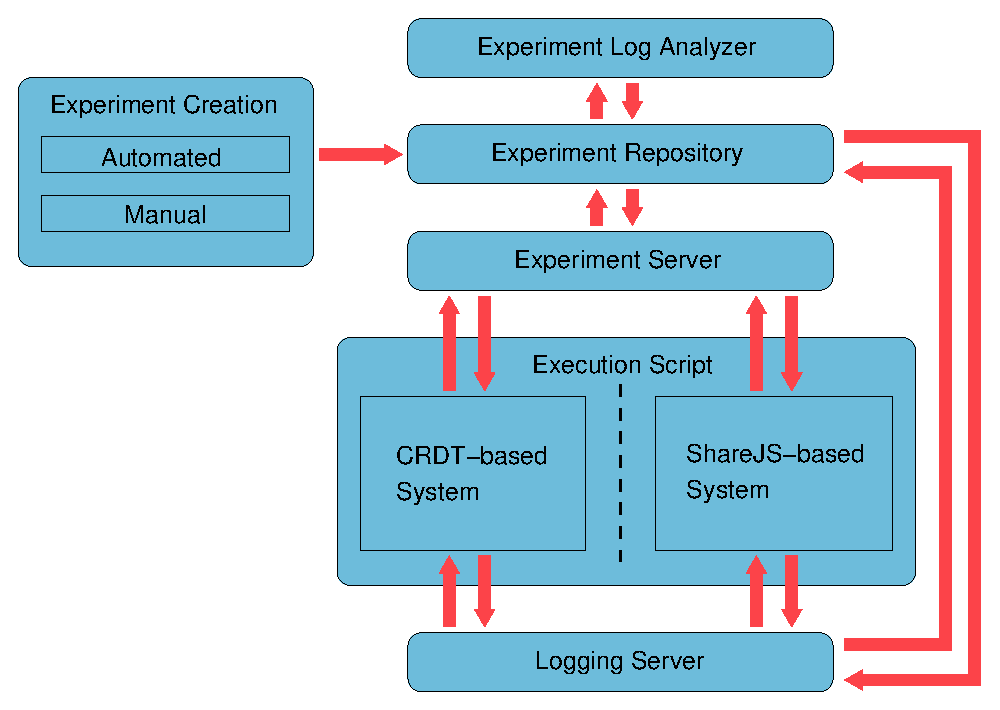
\includegraphics[width=1\linewidth]{figs/workflow.eps}
	\caption[Workflow]{The standard work flow for creating, running, and analyzing experiments.}
	\label{fig:workflow}
	\end{figure}
	
	Manually or with a custom script, experiment setup files are created, with specifications over which variations should be executed (such as different topologies or optimizations enabled). An experiment server provides whichever experiment is queued to the requester, either the CRDT-based system or the ShareJS-based one. In either case, the same basic data is served. The system runs the experiment and submits the resulting log back to a logging server. At some future point, a separate script collects logs and summarizes them into digestible formats. Between experiments, both the testing platform (Google Chrome) and the ShareJS server, if applicable, are relaunched.

	\subsection{Experiment Design}
	
	A basic experiment must define the number of clients participating, a set of events for each client to execute, and the network topology. The events are seeded in the scheduler during an execution. Appendix~\ref{appendix:simpleexpsetup} shows a sample experiment setup in full.

	I decided to assign latencies per-node, and calculate a link latency as the average between two nodes' values, rather than assign per-link because of need to have one network description that fits any topology. This also models the real world better: a device with one high latency link, such as a mobile phone, will likely have only higher latency links rather than some fast and slow links. This ``higher on all connections'' is modeled with an average between a (high-valued) node and its neighbors.

	
	\subsection{Separation of Modeling and Analysis}
	
	Modules for tracing logged packet departures and arrivals end up resembling a set of `clients' and would have fit well into the systems at runtime. However, I decided that having a shared layer that is easily extensible is worth some high level duplication. Another reason is that it is good software engineering: one component should do one task and data creation and analysis are very separate objectives.
	
	An independently running Python script serves this purpose. A sample analysis from a simple experiment is listed in Appendix~\ref{appendix:simplelogsummary}.	
	
	
	
\section{Extension: Local Undo} \label{sec:undo}
	
	In interactive systems undo and redo are key features~\cite{shneiderman1982}. As such, these are interesting extensions to the capabilities of a CRDT for text editing beyond basic insertion and deletion. I chose to implement a local undo --- that is, only allow undoing and redoing operations that were performed locally --- rather than a global undo, where anyone can modify any operation. This is because global undo quickly becomes confusing and counterintuitive during concurrent editing: performing an undo may not affect the user's last operation but unexpectedly revert someone else's. The approaches detailed below were developed originally; one is similar to an implementation I found at a later time in Logoot Undo~\cref{sec:logootundo}.
	
	\subsection{Overview}
	Each client keeps a local stack of operations that it produced. The stack can be truncated to avoid ever-growing memory consumption. To undo an operation, the stack pointer is moved down the stack and the inverse operation of the corresponding item on the stack is generated, executed, and broadcast to other clients.
	
	There are two operations that can be undone or redone: insert and delete. Only one client can ever locally generate an insert event (as each character is tagged with a globally unique identifier generated on the client) and thus only it can undo and redo the operation. However, multiple clients can concurrently delete the same character and so have the same \texttt{delete(node)} operation on their local stack. How this concurrent case is handled leads to two different semantics and consistency models.
	
	
	\subsection{Undo and Redo of Insertions}
	Undo and redo of an insert are not equivalent to deletion and insertion, due to the unique identifiers generated during insertion events. Rather, to satisfy the widely used CCI semantics, a redo must reintroduce the same character with the same unique identifier. The solution to this is discussed in the following subsections.
	
		\subsubsection{Undo/Redo Insert Semantics}
		To satisfy the CCI consistency model and semantics (\cref{sec:cciconsistency}), an undo and a redo should have \textit{the same effect on the visible text as if the prior creation or undo never occurred}. For instance, if $A$ creates a character which is deleted by $B$, and the creation is undone and then redone by $A$, the character should still not be visible: $B$'s delete should take effect as if $A$ never undid the insertion.
		
		This idea leads to the fact that `undo insert' and `delete' operations need to be kept separate. Additionally, `undo insert' needs to take precedence over deletions that have occurred subsequently.
		
		\subsubsection{Implementation}
		
		To achieve the desired functionality, I augmented links in the CRDT with a `visible' tag (denoted $v$). The two new bundles that need to be created are undo-insert and redo-insert, which have the same functional form as undo-delete and redo-delete bundles, and only contain the character identifier to operate upon.
		
		The effect of a undo insert packet on CRDT node $L$ is to set $L.v = false$, while a redo insert packet sets $L.v = true$. When the string is queried from the CRDT (i.e. the CRDT 
		$read()$ method is called), nodes which have $v = false$ are ignored and not retrieved.
		
		As only the originator of an insert can undo and redo it, and therefore only they can access the $v$ flag, conflicting operations can never be produced and there is no need to prove commutativity.
		
	\subsection{Undo and Redo of Deletions}
		Undoing a delete, as mentioned before, is tricker than an insert as multiple clients can concurrently perform and therefore `own' a delete on their local stacks. How this concurrency is handled determines system behavior. The two possibilities are: implementing the CCI consistency model, and a variant I termed ``Immediate Undo'', both presented below.
		
		\subsubsection{CCI Undo/Redo of Deletions} \label{sec:cciundo}
		According to CCI, in the event of an undo delete, the system should behave as if the delete never occurred. So, if users 1 and 2 concurrently delete a character, then 1 undoes its removal, the expected result is that the system behaves as if only the 2's delete happened. While this sounds sensible, it is uncomfortable to user 1: they undid their deletion and expect the character to return. In effect, this consistency model requires \textit{full consensus} between $n$ clients that concurrently deleted a character to return it.
		
			\paragraph{Implementation}
			While consensus is awkward, it is effectively implemented with counters. The key change is to modify the `deleted' tag of links in the CRDT from boolean to integer.
			
\begin{typescript}[New Type Signature of a Link in the CRDT][]
export interface MapEntry {
	c: string,   // character
	n: string,   // next link
	d?: number,  // (optional) deleted, nonexistant $\Rightarrow$ not deleted
	v?: boolean  // (optional) visible, nonexistant $\Rightarrow$ visible
}
\end{typescript}

		%	\paragraph{Delete, Undo, Redo}
			Delete and redo operations increment the $d$ value in the target link. An undo packet has the effect of decrementing $d$.
			
			Now, when the $read()$ method is called on the CRDT, it only retrieves links such that
			
				\[\forall Links\ l.\  (\lnot\exists l.v \lor l.v = true) \land (\lnot\exists l.d \lor l.d = 0 ) \] 
			
			\paragraph{Proof of Commutativity of Delete, Undo, Redo}
			We only need to consider commutativity with other operations that may operate on the same data in the CRDT and therefore conflict. Since any given delete, undo, or redo operation $op$ only affects the specific node $node$ in the linked list identified by $op.deleteId$, the only conflicting operations might be other delete, undo delete, and redo delete operations.
			
			\begin{proof}
				We treat delete and redo delete operations identically, that is having the effect of incrementing $node.d$. An undo delete has the effect of decrementing $node.d$. Any set of these operations applies a sequence of $+1$ and $-1$ to $node.d$. By the commutativity of addition and subtraction, these arithmetic operations can occur in any order, so the delete, undo and redo operations can occur in any order.
			\end{proof}
			
			\paragraph{Cost}
			The cost of this approach is minimal: one extra integer per deleted link in the CRDT.
			
		\subsubsection{Immediate Undo/Redo of Deletions} \label{sec:immediateundo}
		CCI Undo requires users reach consensus to make deleted characters reappear. It would be preferable for any user to be able to immediately undo a character regardless of other users.
		
			\paragraph{Semantics}
			We desire the following semantics:
			
			In the case of conflicting concurrent \textit{make-invisible} operations (such as delete or redo delete) and \textit{make-visible} operations (such as undo delete), the \textit{make-visible} operation will take effect.
			
			This follows from the idea that a user recalling a prior character likely wishes to utilize it, while a user wishing to remove a character does not care about its presence or absence. Note that this effectively inverts the consensus of CCI Undo to require full concurrent agreement to remove a character. 
			
			\paragraph{Implementation}
			In order to support an immediate undo, we need to be able to compare the ``time'' at which a deletion, undo, or redo occurred in order to detect concurrency. Vector clocks allow exactly this. When operations arrive, the packet's vector and the vector stored the relevant CRDT link can be compared and acted upon.
			
			The required modification in the CRDT is that the `deleted' tag $d$ of a CRDT node $l$ now represents a pair ($true/false$, $vector$). The first value is a boolean for whether or not the character is deleted. The second is the result of merging the local vector and the vector of the packet that delivered the operation according to my modified vector clock rules. This executes and returns a pairwise maximum of the two vectors.
			
			As before, delete, undo delete and redo delete bundles contain only the identifier of the node $l$ to act upon. In non-concurrent cases, i.e. a sequence of causally dependent operations, the last operation in the sequence is applied to $l$ (intuitively this is the most recent, non-concurrent one). 
			
			If a remote delete or redo delete operation is concurrent with the merged vector stored in $l.d[1]$, do nothing. This ensures that a local \textit{make-visible} operation retains its effect (e.g. a undo delete). Otherwise, a \textit{make-invisible} operation is already in effect and $l.d[0]$ is already $true$.
			
			Similarly, if a remote undo delete operation is concurrent with the vector stored in $l.d[1]$, always set $l.d$ to $false$, so that the \textit{make-visible} operation takes effect.
			
			In any case, the vector stored at $l.d[1]$ is updated to the current client vector clock.
			
			When the CRDT $read()$ method is called, we only retrieve nodes $l$ in the CRDT that satisfy
			
					\[(\lnot\exists l.v \lor l.v = true) \land (\lnot\exists l.d \lor \lnot l.d[0]) \] 
						
			The proof of commutativity can be found in Appendix \ref{appendix:immundoproof}.
			
			
			\paragraph{Cost} \label{sec:immundo:cost}
			Storing a vector with every character that at one point was deleted can become quite expensive: Vector clocks have size $\Theta (m*log(k))$, where $m$ is the number of clients in the network and $k$ is the decimal length of the longest sequence number in the vector.
			
			One advantage of this approach is that it enables a sort of distributed garbage collection. Every client is known in the network as it cannot become active until requesting a CRDT from a neighbor (\cref{sec:networkjoin}). Clients could record the last known vector sent by every client. Then, they can periodically traverse the local CRDT and remove tombstones whose vectors are strictly older than all the last known vectors of the clients, which guarantees all clients have incorporated the deletion. However the interaction with undo capabilities necessitates further thought and study; this approach is not implemented in this project.
			
			
			\paragraph{Alternative Approaches}
			As seen above, the cost of storing a vector with every deleted element is quite high, though this could be mitigated with vector clock garbage collection. However, it might be preferable to implement similar semantics without vectors. I mentioned before that Immediate Undo in a way inverts consensus to require agreement to make a character disappear. This naturally leads to using counters as in the CCI Undo implementation, but in reverse i.e. counting down from the number of clients in the system rather up from 0. The problem with this approach is that it requires knowledge of how many clients are in the system at all times, and on join or leave all other clients must increment or decrement all counters in tombstones. If a client silently leaves the system, it may never be possible to reach consensus to actually undo or redo a change. This is also an issue present in the CCI Undo implementation.
			
		
	
	\section{Summary of Implementation}
		This chapter described the components I created to evaluate two systems capable of distributed, conflict free text editing. The CRDT-based system was built from the ground up, starting with the conflict-free replicated data type itself. I showed how to optimize it and how to extend its capabilities to include two different forms of undo and redo. To communicate between clients I designed and built a simulated network that guarantees causal delivery, but then also introduced vector clocks to relax requirements on the simulated network. Underlying this network is a scheduler driving the execution of events, some of which are seeded by the experimental setup. The comparative system built around ShareJS executes the same set of events, and the resulting logs from both systems are automatically summarized.


\chapter{Evaluation}
%	This chapter aims to analyze the project's success in terms of meeting the proposed goals.

	\section{Overall Results}
	
	The project can be described as successful if the objectives stated in the proposal are met. These are described below along with brief summaries.
	
	\textbf{Success Criterion 1:} \textit{Implement a concurrent, distributed text editor based on CRDTs.}
	
	I can qualitatively assert that this first goal has been completed, complemented by the data gathered and analyzed below.~\cref{sec:crdt} outlines the components needed and steps taken to create a distributed text editor based on CRDTs with an underlying simulated network. Though the primary use of the editor is to gather data via programmatically predefined experiments, it can also be used interactively via the user interface. This feature is counted towards fulfilling success criterion 1.  $\text{\rlap{$\checkmark$}}\square$
	
	\textbf{Success Criterion 2:} \textit{Pass correctness tests for this CRDT.}
	
	The key property of concurrent, distributed text editing is eventual convergence of the data. To this end, the second success criterion aims to ensure that the implementation provides the same guarantees as the theory. Unit testing of the CRDT helped find and eliminate bugs that broke these guarantees. The successful testing is described more in the following section. $\text{\rlap{$\checkmark$}}\square$
	

	\textbf{Success Criterion 3:} \textit{Obtain and compare quantitative results from ShareJS and the CRDT-based systems}
	
	This criterion was intentionally vague in the proposal to allow maximum flexibility during analysis. The bulk of this chapter will focus on the results obtained by experimenting on both the CRDT and ShareJS based systems.	$\text{\rlap{$\checkmark$}}\square$
	
	
	\section{Testing the CRDT}
	
	The testing of the core CRDT used a \textit{black-box testing} approach~\cite{Patton}. Unit tests were designed for the interface provided by the CRDT without need for knowledge of the CRDT internals. This implies that the CRDT itself could be implemented using a linked list, a linked list within a hash table, or in fact be a completely different CRDT. Insert and delete operations were applied to the CRDT in different orders, and every order needed to produce the same resulting string from \texttt{read()}.
	
	The Typescript unit testing library tsUnit\footnote{\url{https://github.com/Steve-Fenton/tsUnit}} provided the framework used in this process. The testing output is shown below in Figure~\ref{fig:unittests}.

	\begin{figure}[htb]
	\centering
	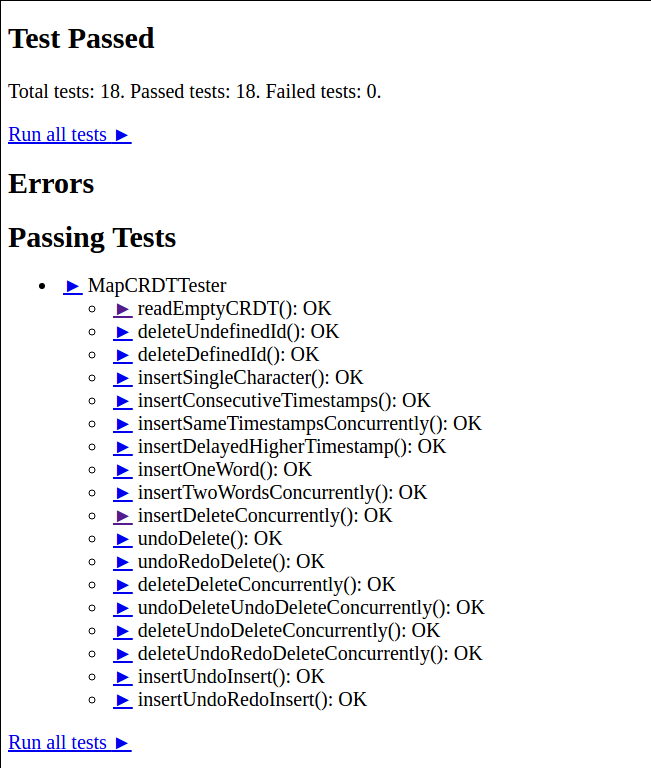
\includegraphics[width=0.56\linewidth]{figs/unittests.png}
	\caption[Unit tests for CRDT]{Results of various unit tests for CRDT. The undo and redo tests depicted here are for the Immediate Undo variant.}
	\label{fig:unittests}
	\end{figure}
	
	
	
	
	\section{Quantitative Analysis} \label{sec:quanteval}
	
		This section aims to empirically test both ShareJS and the underlying operation transformations, and my CRDT-based system. As experiments were run for data collection rather than testing and debugging, the graphical components were disabled: updating the interface is an expensive operation on both systems and impacts results significantly.
		
		
			
		\subsection{Memory}
			Data collected for the following sections was done on the Immediate Undo variant (\cref{sec:immediateundo}) of the CRDT-based system. I averaged results from both star and fully connected networks after determining topology has little affect on memory consumption. The values presented here are the difference between experiment termination and initialization, to only measure the additional memory consumed.
		
			\subsubsection{Sanity Check} \label{sec:sanitycheck}
				As noted in~\cref{sec:sharejs}, I expect both the ShareJS server and clients to suffer from having to save past operations to transform concurrent modifications against. I created a series of experiments which insert and remove the same character a number of times. This ensures that the visible document size is not growing: the only memory growth should be storing past operations. 
				
				For comparison, the same experiments were evaluated on the CRDT system in two ways: firstly using standard insert/delete operations, and secondly as undo/redo operations. The key is that these both have the same effect of inserting and removing characters from the visible document text. However, using insertion and deletion generates a uniquely tagged character each time, so the memory use should increase though the visible document size does not. Doing effectively the same thing with undo and redo operations should not grow internal structures. This test is very useful in establishing the presence of memory leaks and as a general sanity check.
						
						Figure \ref{fig:sanitycheck} confirms these expectations: ShareJS clients and server increase their memory usage as they buffer past operations, though at the end of the experiments the document size is zero characters long. The insert/delete CRDT experiments grow approximately linearly as prediced, whereas using undo/redo shows almost no growth. 
						
										
						This exposes a clear advantage for using CRDT undo/redo versus ShareJS's approach to undo/redo, which generates new operations to undo a prior modification i.e. a delete to undo insertion and an insert to undo a deletion. On the other hand, ShareJS consumes less memory with a static document size and growing number of operations.
								
				\begin{figure}[H]
					\centering
					\includestandalone[mode=buildnew]{data/memory_sanity_check/memory_sanity_check_plot}
					\caption[Memory Consumption Sanity Check] {A plot comparing the performance of the ShareJS client and server, a CRDT-based client performing insertions and deletions, and a CRDT client using undo and redo operations. The error bars indicate one standard deviation from the mean i.e the variation between experiment trials. Deviations in the CRDT data is generally too small to be visible.}
					\label{fig:sanitycheck}
				\end{figure}

		
			\subsubsection{Single Editor} \label{sec:singleeditor}
				In addition to storing past operations, ShareJS components also need to store the document as it grows. This series of experiment explores combined growth with increasing numbers of insertions of single characters. While ShareJS should scale linearly, a CRDT with $n$ characters must store $n$ links of constant size (ignoring deletion requirements), each identified by an identifier of decimal length $log_{10}(n)$, so one might expect a $\Theta (nlog(n))$ space complexity. These experiments were designed using only a single client, inserting only one character at a time,. Results are shown in \ref{fig:sub1}.
					
				To compare to a different workload, another series of experiments was performed inserting words of average length approximately 8 characters rather than individual letters (\ref{fig:sub2}). Both scenarios are plotted on the same axes in \ref{fig:sub3}, with the word insertions rescaled to fit the axis of \ref{fig:sub1}. The data shows that eventually, as the document size becomes very large, ShareJS achieves lower memory consumption. Where this threshold occurs depends on the nature of interactions with the data structures: ShareJS grows less slowly when operations are grouped into fewer, larger packets, reflecting its need to buffer fewer objects in its stack of past operations. On the other hand, my CRDT grows at the same rate no matter what the behavior is (the divergence from 10000 insertions onwards in \ref{fig:sub3} is likely overhead associated with a character by character operations rather than words). 
				
				\begin{figure} [H]
				\centering
				\begin{subfigure}[t]{.45\textwidth}
				  \centering
				  \includestandalone[width=.99\linewidth,mode=buildnew]{data/singleclient_memory/singleclient_plot}
				  \caption[Single Client Memory Consumption with Character Insertion] {A plot of component behavior as characters are inserted one at a time into the documents.}
				  \label{fig:sub1}
				\end{subfigure}%
				\begin{subfigure}[t]{.45\textwidth}
				  \centering
				  \includestandalone[width=.99\linewidth,mode=buildnew]{data/singleclient_word_insert_memory/singleclient_word_insert_plot}
				  \caption{A plot of component behavior as characters are inserted one word at a time. In this scenario, the CRDT overtakes the ShareJS client after approximately 1300 word insertions, or about $1300*7.8 = 10140$ characters.}
				  \label{fig:sub2}
				\end{subfigure}
				\begin{subfigure}[t]{0.6\textwidth}
				  \centering
			  	  \includestandalone[width=1\linewidth,mode=buildnew]{data/combined_single_client_memory/combined_single_client_memory}
				  \caption{A simplified plot including only the ShareJS and CRDT client consumptions on the same axis as \ref{fig:sub1}. The values from \ref{fig:sub2} have been rescaled by the average inserted word length of 7.8 characters.}
				  \label{fig:sub3}
				\end{subfigure}
				\caption[Single Client Memory Consumption]{Plots comparing the behavior of ShareJS and CRDT-based systems under different behaviors.}
				\label{fig:singleclientmemory}
				\end{figure}
				
				To do a high level estimate of which scenario is more likely, I will assume that a person can type at 60 words per minute, words are of average length 5 characters~\cite{bochkarev2012average} and wordwide latencies average 100ms~\cite{latencies}~\cite{fccbroadband}. This leads to about 300 characters per minute, or one character every 200ms. Thus, the character by character streaming scenario that is detrimental to operational transformations is more likely.
					
					
				
				
			\subsubsection{Multiple Clients: Scaling Replication}
				Figure \ref{fig:memvsreplication} examines how both systems scale in terms of the number of connected replicas. In all cases from 1 to 100 connected clients, the CRDT-based distributed editor outperformed the ShareJS based one in terms of overall memory consumption. In the cases of fewer clients, this was by several multiples. Though the CRDT clients appear to exhibit higher aggregate growth as the number of peers increases, part of this can be credited toward overheads in the network simulation.
			
				\begin{figure}[htb]
					\centering
					\includestandalone[mode=buildnew]{data/multiclient_memory/multiclient_plot}
					\caption[Memory Consumption versus Replication] {Combined server and client cost for the ShareJS system next to the CRDT-based system. Error bars represent one standard deviation. Experiments inserted a total of 5000 characters split across the clients. Error bars in the CRDT are generally too small to be visible.}
					\label{fig:memvsreplication}
				\end{figure}
				
			\subsubsection{CRDT System Variants}
				Though the prior data sets were collected with the arguably most useful variation presented in~\cref{sec:immediateundo}, Immediate Undo, in some situations undo functionality may not be necessary, or CCI consistency may be desired. Thus a comparison between the versions developed is worthwhile: Without undo, CCI Undo, and Immediate Undo; ShareJS is tested as well. This series of experiments tests the systems with varying amounts of delete operations, but fixed number of clients (5), insertions (100 words per client) and fixed word length (5 characters), 2500 character insertions in total.
				
				\begin{figure}[htb]
					\centering
					\includestandalone[mode=buildnew]{data/indel_system_compare/indel_system_compare}
					\caption[Behavior of System Variants - Memory] {A plot of the different system variations developed, along with the ShareJS system with a fixed document size and varying number of deletions. Executed with 5 clients, 100 words inserted per client, each word being 5 characters long.}
					\label{fig:variantsmemory}
				\end{figure}
				
				Figure \ref{fig:variantsmemory} shows that not implementing undo provides consistent performance as hardly any data is added into the CRDT, whereas the Immediate Undo variant grows consistently with the number of characters deleted. CCI Undo sits comfortably between the other variants. ShareJS behaves rather unpredictably, but consumes many times more memory than any of the CRDT-based systems, but would likely perform more comparably with a higher number of insertions.
				
			\subsubsection{Summary}
				This subsection explored the behavior of both the ShareJS and CRDT-based systems across a variety of settings. Several key ideas were discovered. Firstly, my CRDT offers significantly better memory consumption for small and medium sized documents, though with large documents and chunked operations tends to perform worse. Secondly, OT, at least in the form used by ShareJS, performs worse when operations are small and frequent, whereas CRDTs' memory consumption is agnostic to the size of operations. Both systems scale relatively similarly as replication increases, though the CRDT generally offered better performance. Lastly, enabling undo functionality has significant overhead, especially when offering `Immediate Undo' semantics, but making effective use of it, perhaps by replacing as many operations with equivalent undo/redo events as possible, can have considerable savings.
					
		\subsection{Network}
			
		
			\subsubsection{Latencies and Batching}
			Figures \ref{fig:latency-cs} and \ref{fig:latency-sc} examine the theoretical speed at which operations can be streamed between ShareJS clients, expecting locally looped back transmissions to be the fastest communication possible. Interestingly, a strange feature of these approximate distributions is the 45ms return time peak in Figure \ref{fig:latency-sc}. I traced this into the implementation of the BrowserChannel\footnote{\url{https://www.npmjs.com/package/browserchannel-middleware}} connection module used by the ShareJS client -- messages actually return within a few milliseconds, but are only made available to the client after an additional delay of about 30-40ms. With a trip time via the server to any other client of at most 50ms, the character streaming limit is about 1200 insertions or deletions before they begin being batched into larger changes.
			
			In comparison my system is more flexible: it can be adjusted to send one character at a time, or buffer and group operations to best match the needs of the larger system (for example, if sending small packets is expensive in the network, it can be programmed to send fewer, larger packets like ShareJS).			
			
			%The data gathered here also helped to generate link latencies for the CRDT network simulation during experiment design. I used the approximately normal distribution from \ref{fig:latency-sc} at 200ms combined with the equivalent distribution in \ref{fig:latency-sc}, which is estimated by a normal with mean 30 and standard deviation 10. These link latencies to an extent determine the amount of concurrency prevalent in the system.
			
			\begin{figure}[H]
				\centering
					\includestandalone[mode=buildnew]{data/latencies/latencies_distributions_client-server}
				\caption[Client-Server Latency] {A plot of client to server latency versus load. Latencies mostly cluster about 3ms until a higher load is generated.}
				\label{fig:latency-cs}
			\end{figure}
			\begin{figure}[H]
				\centering
					\includestandalone[mode=buildnew]{data/latencies/latencies_distributions_server-client}
				\caption[Server-Client Latencies] {A plot of server to client latency versus load. The latencies approach a normal distribution as the load increases.}
				\label{fig:latency-sc}
			\end{figure}
	
		
		\subsubsection{Packet Size}
			The size of packets in both systems is almost fully determined by a few parameters. For this section I will assume that operations are not batched, though they may insert or delete multiple contiguous sequences. As shown above and discussed in~\cref{sec:singleeditor}, in both this testing environment and real world deployments most packets will contain small operations, so this assumption is reasonable.
			
			
			\begin{table}[H]
			\centering
			\caption[ShareJS Insert and Delete Packet Size]{Tabulating the size of ShareJS's insert and delete packets, measured in number of characters required to represent JSON packet as a string.}
			\label{tab:sharepackets}
			\setlength{\tabcolsep}{10pt}
			\begin{tabular}{@{}lll@{}}
                                             & ShareJS Insert             & ShareJS Delete     \\ \toprule
			JSON Overhead (chars)                                      & $25$                       & $25$               \\ \midrule
			Length of string to insert $n$                     & $n$                        & N/A             \\ \midrule
			Number of characters \\to delete $n$                 & N/A                        & $\lfloor log_{10}(n) \rfloor+1$ \\ \midrule
			Position $p$, bounded\\by document size $n_{chars}$ & $\lfloor log_{10}(n_{chars}) \rfloor+1$				 & $\lfloor log_{10}(n_{chars}) \rfloor+1$  \\ \midrule
			Document version $v$, \\bounded by $n_{chars}$       & $\lfloor log_{10}(n_{chars}) \rfloor+1$                 & $\lfloor log_{10}(n_{chars}) \rfloor+1$  \\ \bottomrule
			Total	 		& $27+\boldsymbol{n}+2(\lfloor log_{10}(n_{chars}) \rfloor)$ & \makecell{$28 + \lfloor log_{10}(n)\rfloor + $ \\ $2(\lfloor log_{10}(n_{chars}) \rfloor)$}
			\end{tabular}
			\end{table}	
			
			\begin{table}[H]
			\centering
			\caption[CRDT System Insert Packet Size]{Tabulating the size of the CRDT-based system's insert packets. Delete packets are identical except they do not contain characters to insert and the ID of the character to insert after. Measured in number of characters required to represent JSON packet as a string.}
			\label{tab:crdtinsertpacket}
			\setlength{\tabcolsep}{10pt}
			\begin{tabular}{@{}ll@{}}
			
                             & Cost (upper bound)\\ \toprule                                                                                                                                                       
			JSON Overhead (chars)      & $46$ \\ \midrule
			Client ID                       & $\lfloor log_{10}(n_{clients}) \rfloor+1$  \\ \midrule
			Vector Clock                    & $1 + n_{clients} * (\lfloor log_{10}(n_{operations}) \rfloor + 5)$ \\ \midrule
			Type Disambiguator              & $1$ \\ \midrule
			Characters to Insert            & $n$ \\ \midrule
			ID of First New Character       & $\lfloor log_{10}(n_{chars}) \rfloor + \lfloor log_{10}(n_{clients}) \rfloor  +1$  \\ \midrule
			ID to Insert After & $\lfloor log_{10}(n_{chars}) \rfloor + \lfloor log_{10}(n_{clients}) \rfloor +  1$  \\ \bottomrule
			Total                           & \makecell{$51 + \boldsymbol{n} + \boldsymbol{5n_{clients}} + \boldsymbol{n_{clients} *(\lfloor log_{10}(n_{_{operations}}\rfloor)} +$ \\ $2*(\lfloor log_{10}(n_{chars}) \rfloor + \lfloor log_{10}(n_{clients}) \rfloor)$}
			\end{tabular}
			\end{table}
			
			
			
			The expressions in Tables \ref{tab:sharepackets} and \ref{tab:crdtinsertpacket} are rather complicated but only need to convey a few ideas: Firstly, insert packet sizes scale linearly with the number of characters to add (bolded). Both have significant JSON overheads, though the complexity of the CRDT packets means its overheads are even higher. The vector clock component of the CRDT insert (and delete, not shown here) contributes another $\Theta(nlog(m))$ cost. This reflects the difficulty of routing and enforcing causality in distributed, flexible topology systems. Lastly, the primary components of these expressions that are likely to grow very large are $n_{chars}$, the number of characters in the document, the version $v$ in ShareJS, and $n_{operations}$. However, all of these are present only as $log$ terms, so even large values lead to manageable packet sizes.
			
			Table \ref{tab:samplepacketsizes} shows some typical packet sizes taken from experiments run previously. We see that ShareJS is invariant to the number of clients in the network, whereas the use of vector clocks again penalizes the CRDT-based system. Note that ShareJS packets are shown in two variants: with extraneous meta data stripped out, and with it retained. The meta data allows extra functionality not relevant to this project so should be ignored.
			
			\begin{table}[H]
			\centering
			\caption[Sample Packet Sizes]{Sample Real Packet Sizes, measured in number of characters required to represent JSON packet as a string.}
			\label{tab:samplepacketsizes}
			\setlength{\tabcolsep}{12pt}
			\begin{tabular}{@{}lll@{}}
			Operation													   & 2 Clients & 5 clients \\ \toprule
			ShareJS Insert 5 chars, 30 char document, without metadata & 34        & 34        \\ \midrule
			ShareJS Insert 5 chars, 30 char document, with metadata    & 74        & 74        \\ \midrule
			ShareJS Delete 1 char, 30 char document, without metadata  & 30        & 30        \\ \midrule
			ShareJS Delete 1char, 30 char document, with metadata      & 74        & 74       \\ \midrule
			CRDT Insert 5 chars, 30 char document                      & 70        & 88        \\ \midrule
			CRDT Delete 1 character, 30 char document                  & 54        & 71        \\ \bottomrule

			\end{tabular}
			\end{table}
			
			
			
		\subsubsection{Packet Quantity}
		
			\begin{table}[H]
			\centering
			\caption[Number of Packets in P2P Network] {Table of topology, the number of packets sent per operation, and the time taken until all clients receive the operation the first time. This assumes a constant latency $L$ on each link. The diagrams in the leftmost column demonstrate topologies with $n_{peers}=4$.}
			\label{tab:topologypackets}
			\setlength{\tabcolsep}{10pt}
			\begin{tabular}{@{}lll@{}}
			Topology		& Total Packets Sent            & Time to receipt on all Peers   \\ \toprule
			\makecell{Linear \\ 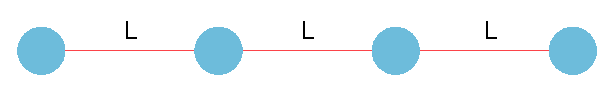
\includegraphics[width=0.15\linewidth]{figs/linear_top.eps}  }        & $n_{peers} - 1$                   & $(n_{peers}-1)L$              \\ \midrule
			\makecell{n-gon  \\ 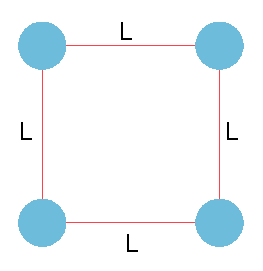
\includegraphics[width=0.15\linewidth]{figs/ngon_top.eps} }        & $n_{peers}+1$                 & $\lfloor n_{peers}/2 \rfloor L$ \\ \midrule
			\makecell{Star  \\ 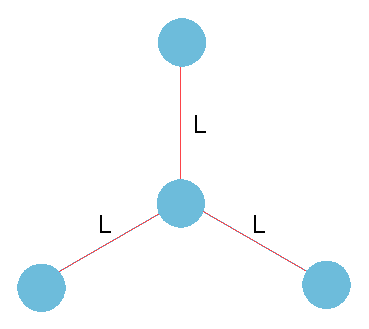
\includegraphics[width=0.15\linewidth]{figs/star.eps} }         & $n_{peers} - 1$ 	                & $2L$                           \\ \midrule
			\makecell{Fully Connected  \\ 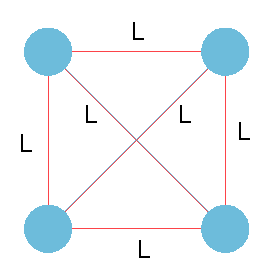
\includegraphics[width=0.15\linewidth]{figs/fullyconnected.eps} } & $n_{peers} * (n_{peers} - 1)$ & $L$                 \\ \bottomrule          
			\end{tabular}
			\end{table}
			
			Routing in a flexible P2P network is more difficult than in a client-server architecture, which is why my system uses a simple broadcast to disseminate packets. However, this becomes more inefficient with increasing connectivity, illustrated in Table \ref{tab:topologypackets}: the number of packets sent approaches a quadratic cost in the number of peers. Connectivity is one major advantage P2P networks have over traditional ones, as it can lower latency, but requires a more sophisticated routing protocol to handle efficiently.
			

			Using a star topology, ShareJS and the CRDT-based system send the same number of packets into the network. However, payloads are usually larger for the CRDT. Additionally, the \textit{average} time for the clients to receive a modification is lower than in ShareJS: the time to the center node is always $L$ rather than $2L$ which brings down the average time for change propagation. However, it would be useful to take advantage of higher connectivity, perhaps using a newer protocol such as Spray~\cite{nedelec2015spray}.
			
			
		\subsubsection{CRDT System Variants}
			As before, in some situations it may not be necessary to use vector clocks to ensure causal delivery. In those cases the basic implementation would work well, and undo functionality could be implemented as CCI Undo (as Immediate Undo must have vector clocks). Figure \ref{fig:sysvariationspackets} demonstrates the cost of using vector clocks once again: packet sizes are double the size versus the basic implementation. ShareJS achieves better performance than any of the CRDT variants.
		
			\begin{figure}[H]
				\centering
				\includestandalone[mode=buildnew]{data/variants_packet_sizes/variants_packet_sizes}
				\caption[Behavior of System Variants - Packet Size] {Cost of insert and delete packets with different system configurations. Both CCI and Immediate Undo variants use identical packets and are shown here as `Undo CRDT' together. ShareJS has very similar insert and delete packet sizes; these are shown together.}
				\label{fig:sysvariationspackets}
			\end{figure}
			
		
		\subsubsection{Summary}
			This section showed that using a CRDT over a P2P network offers flexibility in terms of operation grouping or streaming that ShareJS does not. In addition, on equivalent topologies they send the same quantity of packets, but my system sends packets that are between 1.5 and 3.5 times as large, reflecting the use of P2P networks. Relatedly, using a P2P network can halve the latency to disseminate operations to all peers, but this either comes at the cost of a more complex network protocol or massively increased numbers of packets. Overall, ShareJS generally requires less network capacity and offers reasonable latencies to all clients.
			
		
	
		\subsection{CPU Time}
			Knowing the relative simplicity of CRDT algorithms versus those of OT hints that processing time may be the real benefit of using CRDTs. Especially bad are scenarios where OT has to do costly transformations of incoming operations against a long history of concurrent ones; this issue does not arise with CRDTs, though the worst case scenarios can still be linear in the size of the CRDT.
			
			Unfortunately, web browsers are nonideal platforms for examining computation time (cannot actually measure CPU time). Additionally, nondeterministic latency between ShareJS clients and server could make results unreliable. To handle these issues, I chose to generate very large concurrent operations for both systems and use millisecond-precision timers to measure the time taken from operation arrival from the network until complete integration. Large workloads disguise the use of low precision timers and hide effects of operating system level scheduling. In these experiments, one client is a simple listener and receives operations generated concurrently on other nodes. The times indicated in Figure \ref{fig:cputime} are the sum of processing times on generator nodes, server relay time (if applicable), and integration time on the listener.
			
			As shown in the graph, ShareJS spends much longer generating and integrating changes than the CRDT-based system does. The CRDT operates between 3 and 38 times faster than ShareJS. This data provides strong evidence that CRDTs fare much more favorably under highly concurrent loads. This is in line with what has been found by other authors~\cite{ahmed2011evaluating}.
			
			\begin{figure}[htb]
				\centering
				\includestandalone[mode=buildnew]{data/cpu_testing/cpu_testing}
				\caption[CPU Time] {Comparison between the time taken for both systems to integrate large concurrent edits.}
				\label{fig:cputime}
			\end{figure}		
	
		
		
		
		
		
		


\chapter{Conclusion}

Though realtime collaboration is more feasible than ever, aspects of currently deployable technologies still need improvement. Operational transformations, which power popular services such as Google Docs, are magnitudes slower to integrate concurrent operations and settle into a converged state than alternative CRDT driven approaches. CRDTs are also theoretically simpler and therefore easier to implement without errors. The data- rather than operation-centric approach to eventual consistency utilized by CRDTs allows exploitation of P2P networks, enabling more robust and independent systems to be developed, though this comes at the cost of network traffic and routing complexity. My findings, the apparent stagnation in development of new OT algorithms, and the continuing potential for optimization of CRDTs suggests that future systems will opt for CRDTs over OT for eventual consistency.

%Realtime collaboration is more feasible than ever, with decades of development resulting in mature algorithms based on operational transformations and recently developed CRDTs enabling faster and more efficient distributed applications that conform to users' expectations. This dissertation has compared and contrasted both technologies via implementations of distributed text editors. I gathered evidence that the system I built around a specific CRDT is more efficient in highly concurrent and distributed workloads but needs more work to take advantage of its P2P nature, while ShareJS shows its strengths with very large documents and chunked operations but fares badly under concurrent loads.

\section{Achievements}

I succeeded in meeting all my initial project goals: the final CRDT passed a set of correctness tests I defined, which in turn enabled correct operation of a distributed text editor running on top of a simulated network. To enable comparison, I built a system around the OT enabled ShareJS capable of executing corresponding experiments as my from-scratch editor. In~\cref{sec:quanteval} I presented quantitative analysis exploring various dimensions of both systems: memory usage, network behavior and computation time, across different scales of document sizes and levels of replication. 

In addition to the core goals, I completed one extension which implements two different undo and redo capabilities for the CRDT, each providing different semantics. My work goes beyond that of the creators of the RGA CRDT and makes it as capable as ShareJS for text editing. Data I gathered indicates that implementing the ``Immediate Undo'' semantics has a relatively high cost, but also potential for large savings over the OT approach to undo and redo used in ShareJS.

This project has from the outset been designed to facilitate replacement of the network simulation with a real P2P networking stack. Having this overall goal in mind led me to plan my implementation thoroughly and isolate functionality. The result is a pleasingly modular, extensible piece of engineering that I hope to build on in the future. Aside from the software development perspective, I gained much deeper insight into conflict free algorithms and data structures, reinforced much of the theoretical underpinnings learned in coursework with practical implementation, and discovered how much fun it could be to spend days reading scientific papers and doing real research.

\section{Lessons Learned}
The task of taking an idea and creating a fully fledged, useful implementation is incredibly satisfying. However, with the benefit of hindsight, there are a few adjustments I would make to the development process. I would spend more time focusing on the CRDT, rather than the networking aspect of the project, implementing further optimizations and capabilities. Additionally, getting the network simulation and schedulers working correctly may well have taken just as long as implementing a real network stack and not been worthwhile. Lastly, I underestimated the amount of time it would take to fix memory leaks and complete accurate, comparable evaluations of the systems and would start these steps earlier.


\section{Limitations and Future Work} \label{sec:futurework}

My CRDT is fundamentally a replicated linked list designed specifically for text editing. As such it does not extend particularly well to other sorts of data that might want to be shared, such a JSON. Within the domain of text editing, additional functionality such as copy-paste combined with undo would be difficult, if not impossible, to implement. Only recently have CRDTs been developed which are capable of these block actions~\cite{yu2015crdt}.

However, there remains potential for further work in my system, mostly to do with optimizations.

\begin{itemize}
	\item{\textbf{CRDT Optimizations: } I implemented word insertion at the network level. That is, rather than sending one character with an identifier per packet, sending one word with an identifier only for the first character. This could be extended to the CRDT itself: storing contiguous words compactly and splitting them on demand could reduce the space complexity of the CRDT by many multiples. Other ideas include tombstone garbage collection using vector clocks.}
	
	\item{\textbf{Probabilistic Broadcast: } As discussed previously, flooding is a relatively inefficient delivery mechanism in a P2P network. Instead, a probabilistic broadcast algorithm such as lpbcast combined with an anti-entropy protocol (\cite{eugster2003lightweight}) could be used, reducing the network load while taking advantage of the connectedness of a P2P network. Alternatively a more modern approach such as Spray~\cite{nedelec2015spray} could be used.}

	\item{\textbf{Vector Clocks: } Using full vector clocks overly restricts concurrency as all potentially dependent operations are stalled, rather than only those with real causal requirements. This could be made more efficient by listing dependent operations, again resulting in a form of vector. However, more efficient representations have been developed such as dotted version vectors~\cite{preguicca2010dotted}.}

\end{itemize}



%%%%%%%%%%%%%%%%%%%%%%%%%%%%%%%%%%%%%%%%%%%%%%%%%%%%%%%%%%%%%%%%%%%%%
% the bibliography
\addcontentsline{toc}{chapter}{Bibliography}
\printbibliography

%%%%%%%%%%%%%%%%%%%%%%%%%%%%%%%%%%%%%%%%%%%%%%%%%%%%%%%%%%%%%%%%%%%%%
% the appendices
\appendix

\chapter{Vector Clocks}

\section{Formal Definition}
\label{appendix:vectorclocks}

As outlined in~\cite{fidge1987}, the aim of vector clocks is to implement the $\rightarrow$ relation such that $ a \rightarrow b$ iff $a$ can causally affect $b$. It is possible to have neither $a \rightarrow b$ nor $b \rightarrow a$ indicating concurrent events.

A vector clock $VC$ is an array of integer timestamps $[c_1, c_2...c_n]$. $c_p$ represents last known clock value $c$ of process $p$, 

There are 5 rules associated with traditional vector clocks.
\begin{enumerate}
	\item All values are initially zero.
	\item The local clock value is incremented at least once for each atomic event.
	\item The current value of the entire vector is sent with every outgoing message.
	\item Upon receipt of a vector, set the local vector to be the maximum of corresponding values in the received and local vectors. The local value is incremented by one.
	\item No value is ever decremented.
\end{enumerate}

The desired partial ordering can then be defined

\[VC_a <_v VC_b \leftrightarrow \forall i[VC_a[i] \leq VC_b[i]] \land \exists j[VC_a[j] < VC_b[j]])\]

%\section{Compact Representation}


\section{Modified Vector Clock}
\label{appendix:modifiedvector}

The modified rule used in~\cref{sec:modifiedvectors} changed rule four from the previous section. For completeness, the full modified rules used are listed below.

\begin{enumerate}
	\item All values are initially zero.
	\item The local clock value is incremented with every message sent by a replica.
	\item The current value of the entire vector is sent with every outgoing message.
	\item Upon receipt of a vector, set the local vector to be the maximum of corresponding values in the received and local vectors.
	\item No value is ever decremented.
\end{enumerate}




\chapter{Convergence of Immediate Undo Variant}

\section{Proof of Commutativity} \label{appendix:immundoproof}

Section~\cref{sec:immediateundo} presented an alternative method of implementing undo and redo functionality for the CRDT. To prove convergence, only commutativity needs to be guaranteed as discussed in~\cref{sec:crdtoverview}. The commutativity of the undo and redo operations are presented below.

We only need to consider commutativity with other operations that may operate on the same data in the CRDT and therefore conflict. Since any given delete, undo, or redo operation $op$ only affects the specific node $node$ in the linked list identified by $op.deleteId$, the only conflicting operations might be other delete, undo delete, and redo delete operations.
						
	\begin{proof}
	
	   	Treat delete and redo delete operations identically. Any non-concurrent modifications are not considered as the latest causally dependent operation is defined to take effect.
		
		Take a system which begins in quiescence, submits concurrent operations and returns to quiescence. There are three possible conflicting cases: delete-delete, delete and delete-undo, and undo-undo.
		
		In the delete-delete scenario, the operations are idempotent: both set $node.d[0]$ to $true$ and $node.d[1]$ to the merged local and incoming vectors of the two operations. Thus on any client, the target node is no longer visible. The undo-undo case is exactly analogous except $node.d[0] = false$. 
		
		In the delete, delete-undo case (one client deletes while another deletes then undoes immediately), any client receiving a single delete $op_{d_1}$ first will set $node.d[0] = true$ and record the merged vector in $node.d[1]$. On delivery of the concurrent delete $op_{d_2}$, only the vector at $node.d[1]$ is updated as the node is already marked as deleted. Then, undo $op_{undo_2}$, since it is a \textit{make-visible} operation, and determined to be concurrent with the merged vector stored at $node.d[1]$, takes effect and $node.d[0]$ is set to $false$. If $op_{d_2}$ were delivered before $op_{d_1}$ the same would occur. Lastly, if the first arrivals are $op_{d_2}$ followed by $undo_{d_2}$, the undo takes effect and $node.d[0] = false$ and $node.d[1]$ is set to the merged vector. On arrival of $op_{d_1}$, since it is concurrent with $node.d[1]$ and a \textit{make-invisible} operation taking effect against a \textit{make-visible} operation, it is ignored. Thus, in any case the clients resolve $node.d[0] = false$ and the node is visible. The stored vector is the result of merging the vectors of the three operations. This merge will produce identical results in any order as proven in Lemma \ref{VectorMergeLemma}.
		
	\end{proof}
	
	\begin{lemma}\label{VectorMergeLemma}
		A set of vectors $S = {v_1, v_2... v_n}$ merged in any order will converge to the same result.\\
		The vector merge rule used is Rule 4 from Appendix \ref{appendix:modifiedvector}, which states the merge between vectors $v_a$ and $v_b$ is the component-wise maximum of the vectors. That is, $\forall i. v_{result}^i = max(v_a^i, v_b^i)$.
		
		The result of merging $n$ vectors is $v_{result}^i = max(v_1^i, max(v_2^i,...max(v_{n-1}^i, v_n^i)...))$, though the order of nesting is arbitrary. In any ordering component $i$ is simply the maximum of all possible $i$ components from the set $S$. Thus, the ordering used to merge a set of vectors is irrelevant and produces the same result in any ordering.
		
	\end{lemma}

\chapter{Simple Experiment Experimental Setup and Results}

\section{Experiment Setup}
\label{appendix:simpleexpsetup}

\lstset{
language=C++,
basicstyle=\footnotesize\ttfamily,
commentstyle=\color{red}\ttfamily,
columns=flexible,
breaklines=true
}

\begin{lstlisting}
{
    // Experiment Name
    "experiment_name": "experiment_1", 	
    // How many clients and when they join
    "clients": [0,0,0],		
    // CRDT-only: Per client values used to compute link latencies	
    "network": {				
        "0": {"latency": 196.7632081023716}, 
        "1": {"latency": 220.01040150077455}, 
        "2": {"latency": 122.31541467483453}
    },
    // CRDT-only: type of scheduler to use
    "execution": "event-driven", 	
    // Scheduled events
    "events": {						
        "0": {					// Events for client 0
         "insert": {				// Insert events for client 0
                "0": {				// Insert "coliseums" at time 0, index 0
                    "chars": "coliseums", 
                    "after": 0
                }
            }, 
            "delete": {}			// No delete events
        }, 
        "1": {					// Events for client 1
            "insert": {				// Insert events for client 1
                "15": {				// Insert "tackling" at time 15, index 0
                    "chars": "tackling", 		
                    "after": 0
                }
            }, 
            "delete": {}			// No delete events
        }, 
        "2": {					// Events for client 1
            "insert": {				// Insert events for client 1
                "30": {				// Insert "freshening" at time 30, index 0
                    "chars": "freshening", 
                    "after": 0
                }
            }, 
            "delete": {}			// No delete events
        }
	},
    // CRDT-only: Topologies over which to run the same experiment
    "topology": [					
        "fully-connected", 
        "star"
    ]
}
\end{lstlisting}

\section{Summary of Results of Simple Experiment}
\label{appendix:simplelogsummary}


\begin{lstlisting}
---fully-connected, optimized---
	Total simulation duration: 848.547219206
	Optimizations enabled: True
	All clients converged to same result: True
	Total insert events: 3
	Total delete events: 0
	Total insert packets sent: 13
	Total size of insert packets sent: 1329
	Average insert packet size (incl vector clock etc.): 102.230769231
	Total delete packets sent: 0
	Total size of delete packets sent: 0
	Average delete packet size (incl vector clock etc.): 0
	Expected number of packets sent - given naiive broadcast in a p2p network: 18
	Expected number of packets sent - given optimal p2p network with everyone joining at start: 6
	Latency/wait time per client when requesting CRDT: [0, 416.77360960314616, 319.07862277720614]
	From whom each client request CRDT: [-1, 0, 0]
	Length of stringified document/crdt during state replay, on average: 171
	pre-experiment: 0
	post-topology-init: 149136
	post-graph-init: 1114064
	post-clients-init: 1125632
	post-experiment: -1833488

---star, optimized---
	Total duration: 959.239037182
	Optimizations enabled: True
	All clients converged to same result: True
	Total insert events: 3
	Total delete events: 0
	Total insert packets sent: 9
	Total size of insert packets sent: 917
	Average insert packet size (incl vector clock etc.): 101.888888889
	Total delete packets sent: 0
	Total size of delete packets sent: 0
	Average delete packet size (incl vector clock etc.): 0
	Expected number of packets sent - given naiive broadcast in a p2p network: 12
	Expected number of packets sent - given optimal p2p network with everyone joining at start: 6
	Latency/wait time per client when requesting CRDT: [0, 416.77360960314616, 319.07862277720614]
	From whom each client request CRDT: [-1, 0, 0]
	Length of stringified document/crdt during state replay, on average: 171
	pre-experiment: 0
	post-topology-init: 73776
	post-graph-init: 1485920
	post-clients-init: 1493768
	post-experiment: 1192544

---experiment_1, ot---
	Total simulation duration: 2100.0
	Total insert events: 3
	Total delete events: 0
	Total packets: 18
	Total size of packets sent: 1398
	Average packet payload size: 77.6666666667
	Total size of packets sent, if there were no meta-information: 264
	Average packet payload size without meta-information: 14.6666666667
	Expected number of packets sent - give optimal client-server network with everyone joining at start: 18
	Latency/wait time per client when requesting CRDT: [43.0, 18.0, 19.0, 0]
	From whom each client request CRDT: [-1, -1, -1, -1]
	Length of stringified document/crdt during state replay, on average: 0
	pre-experiment: 0
	post-clients-create: 2170512
	post-clients-init: 716032
	post-experiment: 1101280

\end{lstlisting}

\chapter{Project Proposal}

% Note: this file can be compiled on its own, but is also included by
% diss.tex (using the docmute.sty package to ignore the preamble)
\documentclass[12pt,a4paper,twoside]{article}
\usepackage[pdfborder={0 0 0}]{hyperref}
\usepackage[margin=25mm]{geometry}
\usepackage{graphicx}
\usepackage{parskip}
\begin{document}

\begin{center}
\Large
Computer Science Tripos -- Part II -- Project Proposal\\[4mm]
\LARGE
Conflict Free Document Editing with Different Technologies\\[4mm]

\large
J.~Send, Trinity Hall

Originator: J.~Send

10 October 2016
\end{center}

\vspace{5mm}

\textbf{Project Supervisor:} S.~Kollmann

\textbf{Director of Studies:} Prof.~S.~Moore

\textbf{Project Overseers:} Prof.~T.~Griffin \& Prof.~P.~Lio

% Main document

\section*{Introduction}

\subsection*{Background}

In a world of ever increasing connectivity, collaborative features of applications
will take on greater and greater roles. Popular services such as Google Docs offer real-time
editing of documents by multiple users, a type of interaction that will move from being
a special offering by few applications to a common and expected interface.

The key property that must be implemented to achieve concurrent editing is eventual consistency,
meaning that all connected users should end up with the same result after receiving all changes to the document 
(even if edits conflict). There are two main technologies that are used to enable concurrent editing of a 
document (plain text or otherwise). One approach is Operational Transforms (OT), 
which that generally relies  on having a central server receive, serialize, transform, and 
relay edits occurring simultaneously to each client. OT is notoriously difficult to implement 
correctly as incoming operations have to be transformed against preceding ones on each client, 
such that the result converges. The server may also be required to make some transformations. 
Due to this, central server must be able to read all the operations being performed by clients.
Thus, unless the server is trusted and secure, OT-based services cannot provide any security or privacy guarantees. 

The alternative, newer technology uses Conflict Free Replicated Datatypes (CRDTs). Instead of resolving conflicts and guaranteeing
eventual consistency by transforming operations against each other, CRDTs use special datastructures that guarantee
that no operations will conflict. There are many types of CRDTs that are tailored for different situations. One example
is a simple up-down counter which could be implemented as two locally replicated registers, one for increments and one
for decrements, where the current state is their difference. Compared to OT, there is no interdependence between edits (as long
as the network protocol can guarantee in-order delivery), which means CRDT-based systems can do away with the server
and be implemented using peer to peer (P2P) protocols. This lends itself to security (encryption is now possible between endpoints),
and possibly more scalability and efficiency.

This project is first concerned with exploring and developing a P2P CRDT concurrent text editor, and secondly comparing it to
the OT-based client/server approach available in the open source library ShareJS. Several extensions are also possible,
listed in later sections.

\subsection*{Resources required}

The primary external resource I will need is the library ShareJS, which is published under the MIT license on GitHub.

Additionally, I will be developing on my personal computer, a Thinkpad T440s with 8 GiB of RAM,
128 GB of hard drive space, and a low wattage dual core Intel CPU running at 1.60GHz.
The primary development environment will be under Ubuntu Linux, though Windows 10 is also available 
on the same machine. 

Git with Github will be used as both a version control system and a cloud backup. Dropbox will 
provide continuous cloud backups as well. Backup development machines are any of the MCS computers.

\subsection*{Starting point}

I have some knowledge of the open source library ShareJS from a past internship, which I aim to leverage when 
evaluating and comparing it to my system. My knowledge of CRDTs and the relevant adding/insert/merge
algorithms stems mostly from a high level explanation provided by Martin Kleppmann, along with a diagram.
This will be the starting point for my from-scratch implementation of the concurrent text editor.

Since I have no experience writing test cases and performance profiling, nor network simulation, 
I will have to learn how to do these.

Lastly, I may consult various papers on CRDTs, as well as my supervisor's work in the area, if required.

\section*{Work to be done}

\subsection*{Overview}
I plan to implement a simulation of P2P CRDT text editing using Javascript. Following this, my project will focus on
comparing an existing OT-based concurrent document editing library (ShareJS) to my implementation, in order to draw conclusions
about their relative network and memory efficiency, and scalability. It is highly likely that my 
system will need some optimization, which can feed back into my evaluation and comparison process. In the case that
these phases do not take too long, there are several possible extensions. The first would be to add
a networking layer to the simulation - in effect turning the it into a usable library. The second would be
researching and implementing 'undo' and 'move' operations, which are relatively open research problems.

\subsection*{Detailed Project Structure}

\begin{enumerate}

\item \textbf{Proposal:} Done.

\item \textbf{Core CRDT Development:} Consider and decide on CRDT datastructure. Then detail how I expect
the insert/delete/merge algorithms to work on paper, followed by implementing these. Lastly, I will need to
learn frameworks for testing my implementation. Both hand-coded and automated tests for correctness should be included.

\item \textbf{Implement Simulation:} Model having an arbitrary number of clients each running the CRDT algorithms, and simulate
networking between these clients. Because this is P2P, it may be worth adding functionality for a variety of network
topologies.

\item \textbf{Set up ShareJS and Compare:} Set up the ShareJS environment, mirror functionality and setups 
between two systems as much as possible, and create corresponding performance profiling tests for both 
systems. These will focus on network efficiency, memory usage, and scalability.

\item \textbf{Tune Implementation:} There will likely be opportunity for some optimization, which will
feed back into the performance comparisons in the previous step and help evaluate the optimizations themselves.

\item \textbf{Extensions:} The first extension would be to implement a proper P2P network stack and remove the simulated 
networking. Next would be to research undo and move operations and perhaps try to implement one or both of these.

\end{enumerate}



\subsection*{Possible extensions}

There are two extensions of varying difficulty:

\begin{itemize}

\item (Easier) Replace networking simulation with a P2P networking library. The end result of this extension should be a ready to deploy Javascript library.

\item (Difficult) Research prior work on undo and move functionality using CRDTs. If something suitable is found, implement it. Otherwise, attempt to work toward my own solution.

\end{itemize}


\section*{Success criteria}

These are the main success criteria associated with my project

\begin{enumerate}
\item A concurrent text editor based on CRDTs has been implemented.

\item The concurrent text editor passes all correctness tests.

\item Quantitative results comparing ShareJS and the CRDT based system have been obtained and analyzed.
\end{enumerate}


\section*{Timetable}

Planned starting date is 16/10/2011.

\begin{enumerate}

\item \textbf{Michaelmas weeks 2--3} Develop CRDT datastructure and algorithms on paper. Read into P2P networks 
and simulating them.

\item \textbf{Michaelmas weeks 4--5} Lay out project files and implement network simulation with support for different
P2P topologies.

\item \textbf{Michaelmas weeks 6--8} Implement CRDT datastructures and algorithms, and connect these to network simulation.

\item \textbf{Michaelmas vacation} Learn an appropriate testing framework, write and generate unit tests for correctness of implementation. Fix any bugs discovered by the testing process. Set up ShareJS environment. Begin outlining progress report.

\item \textbf{Lent weeks 0--1} Complete progress report. Mirror functionality of ShareJS to the setup
of my system. Start writing performance benchmarks and scalability tests for both systems.

\item \textbf{Lent weeks 2--4} Execute tests and analyze results. Try to explain differences and similarities observed.
Tune my implementation and evaluate various optimizations. Begin writing dissertation. 

\item \textbf{Lent weeks 5--6} Continue writing dissertation and optimizing system. Begin research for extension
which implements proper networking stack.

\item \textbf{Lent weeks 7--8} Continue writing dissertation. Before terms ends, review and peer-review (including supervisor)
incomplete draft. Implement networking extension. Research undo and move operations with CRDTs.

\item \textbf{Easter vacation:} Finish dissertation draft. Work on undo and move extensions for system.

\item \textbf{Easter term 0--2:} Edit and proof read dissertation. Work on extensions.

\item \textbf{Easter term 3:} Proof read and then submit early to concentrate on exams.

\end{enumerate}


\end{document}


\end{document}
